\documentclass[12pt]{article}
\usepackage[utf8]{inputenc}
\usepackage{graphicx}
\usepackage{booktabs}
\usepackage{hyperref}
\usepackage{geometry}
\geometry{a4paper, left=3.5cm, right=2cm, top=2cm, bottom=2cm}
\usepackage{array}
\usepackage{longtable}
\usepackage{float}
\usepackage{amsmath}
\usepackage{eso-pic}

% Draw a page border on every page
\setlength{\fboxrule}{1.2pt}
\AddToShipoutPictureBG{%
  \put(\LenToUnit{3.0cm},\LenToUnit{1.5cm}){%
    \framebox(\LenToUnit{16.5cm},\LenToUnit{26.7cm}){}%
  }%
}

\begin{document}

% Title Page
\begin{titlepage}
\centering
\vspace*{3cm}
{\Huge \textbf{Carvion AI: Career Development Platform} \par}
\vspace{1.5cm}
{\Large Comprehensive Project Report \par}
\vspace{4cm}
{\large Submitted by: \par}
{\large \textbf{Project Team} \par}
\vfill
{\large \today \par}
\end{titlepage}

\clearpage
\tableofcontents
\clearpage
\clearpage
\section{Abstract}

Carvion AI is a full-stack, AI-powered career development platform designed to assist job seekers in building optimised resumes, discovering personalised career paths, and preparing for job interviews through an integrated suite of intelligent tools. The platform bridges the gap between raw candidate potential and industry-ready readiness by combining modern web technologies with large language model capabilities.

The system is architected as a decoupled web application --- a React (Vite) single-page application on the frontend communicating with a Django REST Framework backend secured via JWT authentication. All primary application data is persisted in MongoDB through the MongoEngine ODM, while session and administrator metadata are managed in SQLite. The AI layer is powered by Google Gemini 2.5 Flash, integrated server-side to provide deterministic, auditable responses.

The platform delivers six core capability domains: Resume Intelligence, which parses uploaded documents, evaluates ATS compatibility scores, and generates detailed improvement reports; AI Career Roadmaps, which produce personalised step-by-step skill acquisition paths aligned to a user's target role; Mock Interview Preparation, an AI-driven simulator that evaluates candidate responses and provides structured feedback; Job and Course Recommendations, a contextual engine that surfaces relevant opportunities and curated learning content; an AI Chatbot Assistant that guides users through platform features in real time; and an Enterprise Admin Console providing real-time KPI dashboards, user lifecycle management, activity audit logs, notification broadcasting, and system health monitoring driven entirely by live backend data.

Security is enforced through role-based access control, custom JWT middleware, request sanitisation, API rate throttling, and centralised rotating log files for application and security events. The platform is designed for production readiness, with graceful AI fallback strategies ensuring service continuity when the AI API is unavailable.

\clearpage
\section{Introduction}

The rapid evolution of the global job market has created a significant demand for intelligent, accessible, and personalised career development tools. Job seekers today face mounting challenges --- from crafting resumes that pass automated screening systems to identifying the precise skills required for competitive roles and demonstrating readiness through structured interview performance. Traditional career support mechanisms, including static resume templates, generalised job boards, and one-size-fits-all guidance resources, are inadequate in addressing the nuanced and dynamic needs of modern candidates.

Carvion AI was conceived to address these gaps through a unified, AI-driven platform that places personalised career intelligence directly in the hands of users. Rather than offering isolated tools, Carvion AI integrates resume analysis, career path generation, interview preparation, job and course discovery, and conversational assistance into a single cohesive experience --- one that adapts to each user's unique profile, goals, and progress.

The platform is built on the premise that artificial intelligence, when applied thoughtfully within a well-engineered software system, can serve as an always-available career mentor. By leveraging large language model capabilities through Google Gemini 2.5 Flash, Carvion AI delivers contextual, actionable, and high-quality guidance that previously required access to professional career coaches or recruiters.

From a technical standpoint, the project presents a practical implementation of a production-grade full-stack web application. The frontend is developed using React with the Vite build toolchain, providing a fast, component-driven user interface. The backend is implemented in Python using Django and Django REST Framework, exposing a RESTful API consumed entirely by the frontend. Data persistence is split across MongoDB, managed through the MongoEngine ODM for user-generated content and AI outputs, and SQLite for administrative and session data. Authentication and authorisation are handled through JWT tokens with role-based access control distinguishing standard users from platform administrators.

The administrative layer of the platform --- the Enterprise Admin Console --- reflects a production-oriented design philosophy. It provides platform operators with real-time visibility into user activity, AI tool usage, system health, and content moderation through live backend data. This ensures that the platform can be governed, monitored, and maintained at scale without reliance on external analytics tooling.

This report documents the design, architecture, implementation, and evaluation of Carvion AI, presenting it as both a practical software engineering project and a meaningful application of applied artificial intelligence to real-world career development challenges.

\clearpage
\section{Motivation}

The motivation behind the development of Carvion AI is deeply rooted in the structural inefficiencies and challenges characteristic of the modern job search landscape. In today’s highly competitive employment market, job seekers must navigate a complex, automated, and often opaque recruitment process. A major hurdle is the widespread adoption of Applicant Tracking Systems (ATS) by employers, which filter out a significant percentage of resumes before they are ever reviewed by a human recruiter. Standard resume builders provide layout templates but offer no feedback on the quality, relevance, or semantic formatting of the content, leaving candidates in a feedback loop of silent rejections.

Furthermore, the career preparation journey is highly fragmented. Candidates are forced to use multiple, disconnected tools: drafting resumes on one site, seeking job listings on another, searching for online classes to fill skill gaps on third-party libraries, and practicing for interviews on standalone coding or behavioral Q&A platforms. This fragmentation results in a loss of unified career context, forcing candidates to repeatedly re-enter their profiles and goals.

Professional, personalized career mentoring and mock interview coaching are highly effective in addressing these issues, but they are expensive, time-consuming, and inaccessible to the vast majority of job seekers. This financial and resource barrier disproportionately affects early-career professionals and career switchers.

Carvion AI was designed to democratize access to high-quality career mentoring. By integrating resume intelligence, automated ATS scoring, dynamic learning path generation, interactive mock interviews, and conversational career support into a single, cohesive, and context-aware platform powered by Google Gemini 2.5 Flash, the project aims to replace a series of repetitive, isolated tasks with a continuous, guided career development cycle.

\clearpage
\section{Objectives}

The primary objectives of the Carvion AI project are as follows:

\begin{enumerate}
  \item \textbf{To develop an AI-powered resume analysis system} that parses user-uploaded resumes, extracts structured information, evaluates ATS compatibility scores, and generates actionable improvement recommendations using large language model capabilities.

  \item \textbf{To implement a personalised career roadmap generator} that produces step-by-step learning paths, skill acquisition targets, and milestone guidance tailored to each user's current profile and desired career destination.

  \item \textbf{To build an AI-driven mock interview simulator} that presents role-specific questions, evaluates candidate responses in natural language, and delivers structured feedback to improve both technical and communication readiness.

  \item \textbf{To create an intelligent job and course recommendation engine} that surfaces relevant opportunities and curated learning resources aligned to a user's skills, goals, and platform activity history.

  \item \textbf{To integrate a conversational AI assistant} embedded across the platform that answers career queries, contextualises resume feedback, and guides users through platform features in real time.

  \item \textbf{To design and implement a secure, role-based authentication system} using JWT tokens that clearly separates standard user access from administrator privileges, ensuring data privacy and platform integrity.

  \item \textbf{To engineer a production-grade Enterprise Admin Console} that gives platform operators live visibility into user activity, AI tool usage, content moderation, system health, and operational KPIs --- all driven by real backend data with no hardcoded values.

  \item \textbf{To apply modern full-stack web engineering practices} by building a decoupled architecture --- a React (Vite) single-page application on the frontend and a Django REST Framework API on the backend --- connected through a well-defined RESTful interface.

  \item \textbf{To ensure platform reliability and security} through request sanitisation, API rate throttling, maintenance mode management, centralised rotating log files, and graceful AI fallback strategies that maintain service continuity when the AI API is unavailable.

  \item \textbf{To deliver a premium, accessible, and responsive user experience} that removes barriers to professional career guidance and makes AI-powered career development available to any user regardless of background or location.
\end{enumerate}

\clearpage
\section{Existing System}

The existing landscape of career development tools is fragmented and largely reliant on static, non-adaptive resources. Current solutions available to job seekers typically fall into one or more of the following categories:

\textbf{Resume Builders and Templates} --- Platforms such as Canva, Zety, and Novoresume allow users to construct resumes using pre-designed templates. While visually capable, these tools offer no intelligence layer. They do not evaluate content quality, assess ATS compatibility, or provide feedback on how a resume performs against a specific job description. The user receives a formatted document with no understanding of whether it will succeed in an automated screening process.

\textbf{Job Boards} --- Platforms such as LinkedIn, Indeed, and Naukri aggregate job listings and allow users to apply directly. However, they do not analyse a candidate's readiness for a given role, do not recommend skill gaps to address, and do not guide users through the preparation process. The application experience is transactional rather than developmental.

\textbf{Online Learning Platforms} --- Platforms such as Coursera, Udemy, and edX provide course libraries but require users to independently determine what they need to learn. There is no contextual mapping between a user's current skills and their target role, nor any integration between learning activity and resume or interview readiness.

\textbf{Interview Preparation Tools} --- Standalone tools such as Pramp and Interview Cake focus exclusively on technical interview preparation, primarily for software engineering roles. They do not integrate with a user's resume or career profile, and they do not provide AI-evaluated feedback on free-form responses.

\textbf{Limitations of the Existing System:}

\begin{itemize}
  \item Tools are isolated --- resume, job search, learning, and interview preparation exist in separate platforms with no shared context.
  \item No personalisation --- guidance is generic and not adapted to a user's specific background, target role, or skill level.
  \item No AI analysis --- resume and interview feedback, where available, is rule-based or human-driven rather than intelligent and scalable.
  \item No administrative oversight --- existing consumer tools provide no enterprise-grade management layer for organisations deploying these tools at scale.
  \item Fragmented user experience --- candidates must manage multiple accounts, tools, and workflows to accomplish what a unified platform could deliver in one place.
\end{itemize}

\clearpage
\section{Proposed System}

Carvion AI proposes a unified, intelligent career development platform that consolidates all career-related capabilities under a single, AI-driven environment. The proposed system directly addresses every limitation identified in the existing landscape.

\textbf{Unified Platform Architecture} --- Carvion AI integrates resume analysis, career roadmap generation, mock interview preparation, job and course recommendations, and conversational AI assistance within a single application. Users maintain one profile that informs all platform features, eliminating the need to manage multiple disconnected tools.

\textbf{AI-Powered Resume Intelligence} --- The platform accepts resume uploads in PDF and DOCX formats, parses document content using PyMuPDF and python-docx, and extracts structured data including experience, education, skills, projects, and certifications. Google Gemini 2.5 Flash then evaluates the extracted content against industry standards, produces an ATS compatibility score, and generates a detailed, actionable improvement report specific to the user's profile.

\textbf{Personalised Career Roadmaps} --- Based on a user's current skills and their stated target role, the system generates a structured, step-by-step learning roadmap. Each roadmap includes skill milestones, recommended learning resources, and estimated progression timelines --- all produced dynamically through AI inference rather than static templates.

\textbf{Mock Interview Simulator} --- Users can engage in AI-driven interview sessions tailored to their target role. The system presents contextually relevant questions, processes free-form candidate responses, and delivers structured feedback covering content quality, communication clarity, and areas for improvement. This makes professional-grade interview preparation scalable and continuously available.

\textbf{Contextual Recommendations Engine} --- The platform surfaces job opportunities and learning courses that are relevant to each user's skills, career goals, and activity history. Recommendations are contextual rather than keyword-based, improving relevance and reducing discovery effort.

\textbf{Conversational AI Assistant} --- An embedded chatbot assistant is available across the platform to answer career-related queries, explain resume feedback, and guide users through features in natural language. This removes friction from the user experience and provides always-available support.

\textbf{Enterprise Admin Console} --- Platform administrators are provided a dedicated management environment with real-time KPI dashboards, user lifecycle management, AI tool usage monitoring, activity audit logs, notification broadcasting, and system health indicators --- all driven by live backend data. This enables scalable platform governance without reliance on third-party analytics tools.

\textbf{Security and Reliability} --- The proposed system implements JWT-based authentication, role-based access control, API rate throttling, request sanitisation, maintenance mode management, and centralised rotating log files. Graceful AI fallback strategies ensure that core platform functions remain available even when the external AI API is unreachable.

\textbf{Advantages of the Proposed System over Existing Systems:}

\begin{itemize}
  \item A single platform replaces multiple fragmented tools.
  \item All features are contextually connected through a shared user profile.
  \item AI-generated feedback is personalised, scalable, and continuously available.
  \item Career development is treated as an end-to-end journey rather than a series of isolated tasks.
  \item The platform is production-ready with a full administrative oversight layer.
  \item No dependency on external analytics ---  all metrics are computed from live backend data.
\end{itemize}

\clearpage
\section{Feasibility Study}

To evaluate the operational and economic viability of the Carvion AI platform, a comprehensive feasibility study was conducted across three primary dimensions: technical, operational, and economic feasibility.

\begin{itemize}
  \item \textbf{Technical Feasibility:} The technical architecture of Carvion AI utilizes a modern, decoupled stack built on robust, industry-standard frameworks. The frontend is powered by React (Vite) and styled with Vanilla CSS, which provides a fast, responsive, and responsive user interface with low load times. The backend is implemented using Django and Django REST Framework, which offers built-in security features, URL routing, and a clean RESTful interface for client communication. For data storage, MongoDB serves as the primary document store, managed via the MongoEngine ODM. This is highly suitable for handling the nested, complex, and variable JSON schemas generated by the Google Gemini API (such as roadmaps, interview transcripts, and ATS feedback reports), which would be difficult to store in a rigid relational database. Relational metadata, such as Django sessions and JWT blacklists, are efficiently handled by SQLite. The server-side integration of the Google Gemini 2.5 Flash API ensures secure, fast, and reliable AI inference. The local PDF and DOCX parsers (PyMuPDF and python-docx) run efficiently within the Python environment. Thus, the system is technically feasible.
  \item \textbf{Operational Feasibility:} Operational feasibility determines how well the system will fit into the workflow of its target users and administrators. Carvion AI includes a robust Enterprise Admin Console that provides administrators with real-time KPI metrics, user management controls, notification broadcasting, and system health status. The console computes metrics dynamically from live database queries, ensuring administrative decisions are based on accurate data. For reliability, the system features graceful fallback mechanisms to handle external API outages, returning default feedback rather than crashing the interface. Throttling and rate-limiting protect high-cost endpoints from abuse. Because the platform automates resume analysis and interview simulations, it requires very little daily administrative supervision.
  \item \textbf{Economic Feasibility:} The economic feasibility highlights the cost-effectiveness and scalability of the platform. The system relies entirely on open-source databases and software frameworks, eliminating licensing costs. By executing the AI logic server-side via the Google Gemini API, the platform operates on a pay-as-you-go model, minimizing server overhead. The automated nature of the resume checking, roadmap generation, and mock interview evaluation features allows the platform to serve thousands of concurrent users without scaling up human staff or advisors. The low ongoing infrastructure costs, combined with the high value delivered to job seekers, make Carvion AI highly economically feasible.
\end{itemize}

\clearpage
\section{Methodology}

The development of the Carvion AI platform was structured around the Agile Software Development Life Cycle (SDLC) to support iterative refinement, modular integration, and flexibility in response to testing feedback. The methodology was divided into five distinct phases:

\begin{enumerate}
  \item \textbf{Requirements Gathering and Analysis:} During this initial phase, the project requirements were categorized into functional requirements (such as JWT authentication, resume parsing, roadmap generation, mock interviews, job recommendations, and administrative controls) and non-functional requirements (including security parameters, API rate limits, response times, and database consistency).
  \item \textbf{System Architecture and Database Design:} This phase focused on defining the decoupled client-server architecture. System boundaries and data flows were mapped using Data Flow Diagrams (DFD) across multiple detail levels (Levels 0 to 3). Database modeling was performed to map JSON structures to MongoDB collections, defining references, indexes, and cascade deletion rules to maintain database integrity.
  \item \textbf{Iterative Development and API Integration:} Backend development began with setting up the Django REST Framework project and writing models for user profiles and sessions. The local text parsers (PyMuPDF for PDF and python-docx for DOCX files) were integrated, and prompt templates were designed to invoke the Google Gemini API. Once backend views were operational, frontend development proceeded with React, assembling the components, configuring Axios interceptors for automatic JWT header attachments, and integrating TanStack Query for state synchronization.
  \item \textbf{Testing and Quality Assurance:} A comprehensive testing matrix was executed. Unit tests verified individual functions like token validation and text extraction. Integration tests checked client-server data synchronization. System tests validated end-to-end workflows (e.g., uploading a resume and verifying the resulting ATS score update on the dashboard). Finally, security testing checked token blacklisting, and performance testing optimized database indexes.
  \item \textbf{Deployment and Maintenance Planning:} The platform was structured for operational stability by configuring Python's rotating file logging to monitor security and application events. Administrative overrides, such as cache flushing and maintenance mode toggling, were built directly into the operational console.
\end{enumerate}

\clearpage
\section{Requirements}

\subsection{Functional Requirements}

\textbf{User Authentication and Account Management}

\begin{itemize}
  \item The system shall allow users to register an account using a valid email address and a secure password.
  \item The system shall authenticate users using JSON Web Tokens (JWT) with access and refresh token mechanisms.
  \item The system shall support password change and account profile update operations.
  \item The system shall enforce role-based access control, distinguishing standard users from platform administrators.
  \item The system shall restrict all protected routes and API endpoints to authenticated users only.
\end{itemize}

\textbf{Resume Management}

\begin{itemize}
  \item The system shall allow users to upload resumes in PDF and DOCX formats.
  \item The system shall parse uploaded documents and extract structured data including personal details, work experience, education, skills, projects, and certifications.
  \item The system shall evaluate each resume for ATS compatibility and produce a numerical score.
  \item The system shall generate a detailed AI-powered improvement report identifying weaknesses and recommending specific enhancements.
  \item The system shall store all resume data and analysis results persistently against the user's profile.
  \item The system shall allow users to view, update, and delete their stored resumes.
\end{itemize}

\textbf{Career Roadmap Generation}

\begin{itemize}
  \item The system shall allow users to input their current skills and a target job role.
  \item The system shall generate a personalised, step-by-step career learning roadmap using AI inference.
  \item The system shall include skill milestones, recommended learning resources, and progression guidance within each roadmap.
  \item The system shall store generated roadmaps and allow users to revisit them at any time.
\end{itemize}

\textbf{Mock Interview Preparation}

\begin{itemize}
  \item The system shall present users with role-specific interview questions tailored to their stated target position.
  \item The system shall accept and evaluate free-form user responses using AI analysis.
  \item The system shall return structured feedback covering content relevance, communication quality, and areas requiring improvement.
  \item The system shall maintain a history of completed interview sessions accessible to the user.
\end{itemize}

\textbf{Job and Course Recommendations}

\begin{itemize}
  \item The system shall surface job opportunities relevant to the user's skills, target role, and activity history.
  \item The system shall recommend learning courses aligned to identified skill gaps and career goals.
  \item The system shall allow users to save job listings and courses to their profile for later reference.
\end{itemize}

\textbf{AI Chatbot Assistant}

\begin{itemize}
  \item The system shall provide a conversational AI assistant accessible from all primary pages of the platform.
  \item The assistant shall answer career-related queries, explain resume feedback, and guide users through platform features.
  \item The system shall maintain session context within an active conversation.
\end{itemize}

\textbf{Enterprise Admin Console}

\begin{itemize}
  \item The system shall provide administrators with a dedicated login and restricted access environment.
  \item The system shall display a real-time executive dashboard presenting platform KPIs, system health, AI usage, and active alerts derived entirely from live backend data.
  \item The system shall allow administrators to view, search, filter, and manage all standard user accounts.
  \item The system shall allow administrators to view, moderate, and respond to contact messages submitted by users.
  \item The system shall allow administrators to broadcast notifications to selected users or all users.
  \item The system shall log all significant administrator actions in an auditable activity log with timestamps, actor identification, and event descriptions.
  \item The system shall provide administrators with analytics charts covering user growth, AI tool usage, resume activity, and engagement trends.
  \item The system shall allow administrators to flush application cache and manage platform maintenance mode.
\end{itemize}

\noindent\rule{\textwidth}{0.4pt}

\subsection{Non-Functional Requirements}

\textbf{Performance}

\begin{itemize}
  \item The system shall return API responses for standard user operations within 2 seconds under normal load conditions.
  \item The AI-powered operations, including resume analysis and roadmap generation, shall complete within 15 seconds and present appropriate loading indicators to the user during processing.
  \item The frontend application shall load the initial page within 3 seconds on a standard broadband connection.
\end{itemize}

\textbf{Security}

\begin{itemize}
  \item All API endpoints shall require valid JWT authentication tokens except public registration and login endpoints.
  \item Passwords shall be stored as cryptographic hashes and never transmitted or stored in plain text.
  \item The system shall sanitise all user inputs on the backend to prevent injection and malformed data attacks.
  \item API rate throttling shall be applied to prevent abuse of high-cost endpoints.
  \item All application and security events shall be written to rotating log files maintained on the server.
\end{itemize}

\textbf{Scalability}

\begin{itemize}
  \item The backend architecture shall be stateless, enabling horizontal scaling of the API server without session dependency.
  \item MongoDB shall be used for all user-generated content and AI outputs, supporting flexible schema evolution as platform features expand.
\end{itemize}

\textbf{Reliability}

\begin{itemize}
  \item The system shall implement graceful AI fallback strategies that preserve core platform functionality when the Google Gemini API is unavailable or returns an error.
  \item The system shall handle backend exceptions gracefully and return informative error responses to the frontend without exposing internal system details.
\end{itemize}

\textbf{Usability}

\begin{itemize}
  \item The user interface shall be fully responsive and functional across desktop, tablet, and mobile screen sizes.
  \item All interactive elements shall provide visual feedback, including loading states, success confirmations, and error messages.
  \item The platform shall support both light and dark display modes.
\end{itemize}

\textbf{Maintainability}

\begin{itemize}
  \item The backend shall be organised into clearly separated Django applications, each responsible for a distinct domain.
  \item The frontend shall follow a feature-based component architecture, separating concerns between pages, components, and API service layers.
  \item All significant administrator operations shall be auditable through the activity log system without requiring direct database inspection.
\end{itemize}

\textbf{Compatibility}

\begin{itemize}
  \item The frontend application shall be compatible with current versions of Google Chrome, Mozilla Firefox, Microsoft Edge, and Safari.
  \item The backend API shall conform to RESTful conventions, returning JSON-formatted responses with appropriate HTTP status codes.
\end{itemize}

\clearpage
\section{Technologies Used}

\subsection{Frontend}

\textbf{React (v18)} --- The primary frontend library used to build the user interface as a component-based single-page application. React's declarative rendering model enables efficient UI updates and a modular codebase structure.

\textbf{Vite} --- The build toolchain and development server for the frontend application. Vite provides near-instant hot module replacement during development and optimised production builds through native ES module support.

\textbf{React Router DOM} --- Used for client-side routing, enabling navigation between platform pages without full-page reloads while preserving browser history and enabling protected route enforcement.

\textbf{TanStack Query (React Query)} --- Used for server state management, data fetching, caching, and background synchronisation between the frontend and the Django REST API. Simplifies loading and error state handling across all data-dependent components.

\textbf{Recharts} --- A composable charting library built on SVG used to render analytics charts and dashboard visualisations, including line charts, bar charts, pie charts, and area charts.

\textbf{React Icons (Feather Icons)} --- Icon library providing consistent, lightweight SVG icons used throughout the interface for navigation, KPI cards, status indicators, and interactive controls.

\textbf{Axios} --- HTTP client used to make all API requests from the frontend to the backend, with interceptors configured for automatic JWT token attachment and refresh token handling.

\textbf{Vanilla CSS} --- Custom CSS used for all styling including layout, animations, dark mode, glassmorphism effects, and component-level design tokens. No CSS framework dependency.

\noindent\rule{\textwidth}{0.4pt}

\subsection{Backend}

\textbf{Python (v3.11)} --- The primary programming language for all backend logic, including API views, business logic, AI integration, document parsing, and security middleware.

\textbf{Django (v4.x)} --- The web framework underpinning the backend application. Django provides the project structure, ORM for SQLite operations, authentication foundations, admin scaffolding, and application configuration.

\textbf{Django REST Framework (DRF)} --- The toolkit used to build the RESTful API consumed by the frontend. DRF handles serialisation, view routing, authentication classes, permission classes, and API throttling.

\textbf{Simple JWT} --- Django REST Framework extension providing JSON Web Token authentication with configurable access token lifetimes, refresh token rotation, and token blacklisting on logout.

\textbf{MongoEngine} --- An Object Document Mapper (ODM) used to interface with MongoDB from Django. All user-generated content including resumes, AI outputs, roadmaps, interview sessions, jobs, and courses are modelled as MongoEngine documents.

\textbf{PyMuPDF (fitz)} --- Python library used to parse PDF resume uploads, extract raw text content page by page for downstream AI processing.

\textbf{python-docx} --- Python library used to extract text content from DOCX format resume uploads, supporting paragraph-level text extraction.

\textbf{Google Generative AI SDK (google-generativeai)} --- The official Python SDK used to interface with Google Gemini 2.5 Flash. All AI-powered features including resume analysis, career roadmap generation, interview question generation, response evaluation, and chatbot responses are processed through this SDK.

\textbf{django-cors-headers} --- Middleware handling Cross-Origin Resource Sharing (CORS) headers, permitting the React frontend served from a different origin to communicate with the Django API during development and production.

\textbf{Python Logging (RotatingFileHandler)} --- Standard library logging module configured with rotating file handlers to write application events and security events to persistent log files with automatic size-based rotation.

\noindent\rule{\textwidth}{0.4pt}

\subsection{Database}

\textbf{MongoDB} --- The primary document database used for all user-generated content and AI outputs. MongoDB's flexible schema supports the varied and evolving document structures produced by AI analysis, resume parsing, roadmap generation, and interview session data. Accessed through MongoEngine.

\textbf{SQLite} --- The relational database used by Django's built-in ORM for administrator accounts, session management, JWT token blacklisting, and Django admin metadata. Suitable for the administrative data layer given its low concurrency requirements.

\noindent\rule{\textwidth}{0.4pt}

\subsection{AI and Machine Learning}

\textbf{Google Gemini 2.5 Flash} --- The large language model powering all AI capabilities within the platform. Gemini 2.5 Flash was selected for its balance of inference speed, output quality, and cost efficiency for high-frequency API operations. It is used for resume analysis and improvement reports, ATS scoring, career roadmap generation, mock interview question generation and response evaluation, chatbot conversation handling, and contextual career advice.

\noindent\rule{\textwidth}{0.4pt}

\subsection{Development Tools}

\textbf{Visual Studio Code} --- Primary code editor used for frontend and backend development.

\textbf{Git} --- Version control system used to track all source code changes throughout the development lifecycle.

\textbf{Postman} --- Used during development to test and validate all backend API endpoints independently of the frontend application.
\textbf{Visual Studio Code} --- Primary code editor used for frontend and backend development.

\textbf{Git} --- Version control system used to track all source code changes throughout the development lifecycle.

\textbf{Postman} --- Used during development to test and validate all backend API endpoints independently of the frontend application.

\textbf{npm} --- Node package manager used to install, manage, and run frontend dependencies and development scripts.

\textbf{pip} --- Python package installer used to manage all backend library dependencies declared in `requirements.txt`.

\textbf{PowerShell} --- Shell environment used to run backend and frontend development servers on Windows during the development phase.


\clearpage
\section{Data Flow Diagrams}

\subsection{DFD Symbols}


\begin{longtable}{|p{0.22\textwidth}|p{0.25\textwidth}|p{0.45\textwidth}|}
\hline
\textbf{Symbol} & \textbf{Shape} & \textbf{Meaning} \\ \hline
\endhead
\textbf{External Entity} & Rectangle & A person or system outside the system boundary that inputs or receives data \\ \hline
\textbf{Process} & Rounded Rectangle & A function that transforms input data into output data. Numbered for reference. \\ \hline
\textbf{Data Store} & Open Rectangle (two parallel lines) & Persistent storage such as a database, file, or repository \\ \hline
\textbf{Data Flow} & Labelled Arrow & Movement of data between entities, processes, and stores \\ \hline
\end{longtable}


\noindent\rule{\textwidth}{0.4pt}

\subsection{Level 0 — Context Diagram}

The context diagram shows the entire Carvion AI platform as a single process (Process 0) surrounded by all external entities and high-level data flows between them.

\begin{figure}[H]
  \centering
  
\includegraphics[width=0.9\textwidth]{dfd_level0.png}
  \caption{DFD Level 0 - Context Diagram}
\end{figure}

\textbf{External Entities:}
\begin{itemize}
  \item \textbf{USER (Job Seeker)} — Registers, logs in, uploads resumes, requests roadmaps and interviews, receives AI-generated results.
  \item \textbf{ADMINISTRATOR} — Manages users, monitors platform health, reviews audit logs, broadcasts notifications.
  \item \textbf{Google Gemini 2.5 Flash API} — External AI service that receives structured prompts and returns intelligent responses.
\end{itemize}

\noindent\rule{\textwidth}{0.4pt}

\subsection{Level 1 — Main System Processes}

Level 1 decomposes the single Carvion AI process into its six major functional sub-processes and shows all primary data stores.

\begin{figure}[H]
  \centering
  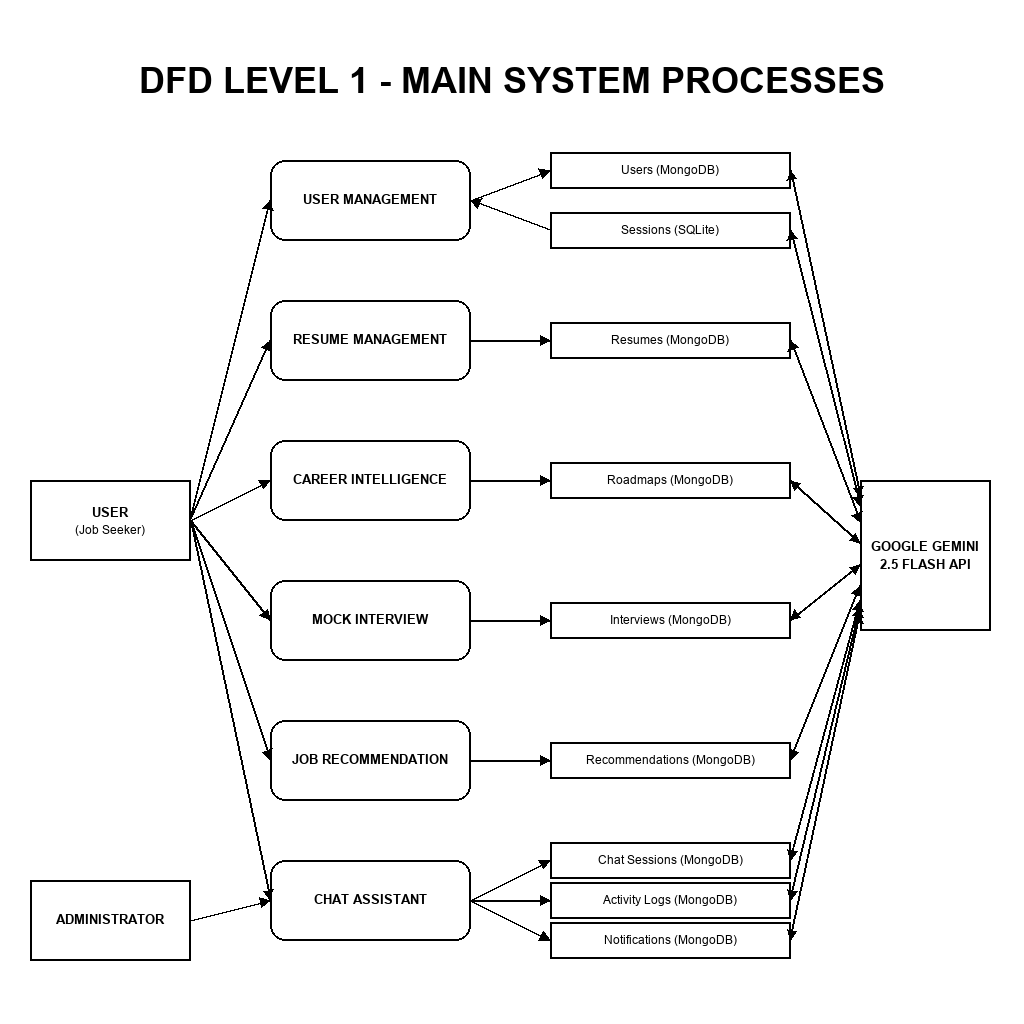
\includegraphics[width=0.9\textwidth]{dfd_level1.png}
  \caption{DFD Level 1 - Main System Processes}
\end{figure}

\textbf{Data Stores:}


\begin{longtable}{|p{0.18\textwidth}|p{0.20\textwidth}|p{0.15\textwidth}|p{0.39\textwidth}|}
\hline
\textbf{ID} & \textbf{Name} & \textbf{Database} & \textbf{Content} \\ \hline
\endhead
D1 & Users & MongoDB & User accounts, roles, profile data \\ \hline
D2 & Sessions / Auth Tokens & SQLite & JWT blacklist, Django session data \\ \hline
D3 & Resumes & MongoDB & Resume documents, parsed data, ATS scores, AI reports \\ \hline
D4 & Roadmaps & MongoDB & Generated career learning roadmaps \\ \hline
D5 & Interviews & MongoDB & Interview sessions, questions, responses, feedback \\ \hline
D6 & Recommendations & MongoDB & Saved jobs, courses, recommendation history \\ \hline
D7 & Chat Sessions & MongoDB & Chatbot conversation history \\ \hline
D8 & Activity Logs & MongoDB & Admin audit trail records \\ \hline
D9 & Notifications & MongoDB & Platform notifications and broadcasts \\ \hline
\end{longtable}


\noindent\rule{\textwidth}{0.4pt}

\subsection{Level 2 — Process Decomposition}

Level 2 decomposes the Resume Management process (Process 2.0) into its detailed internal sub-processes.

\begin{figure}[H]
  \centering
  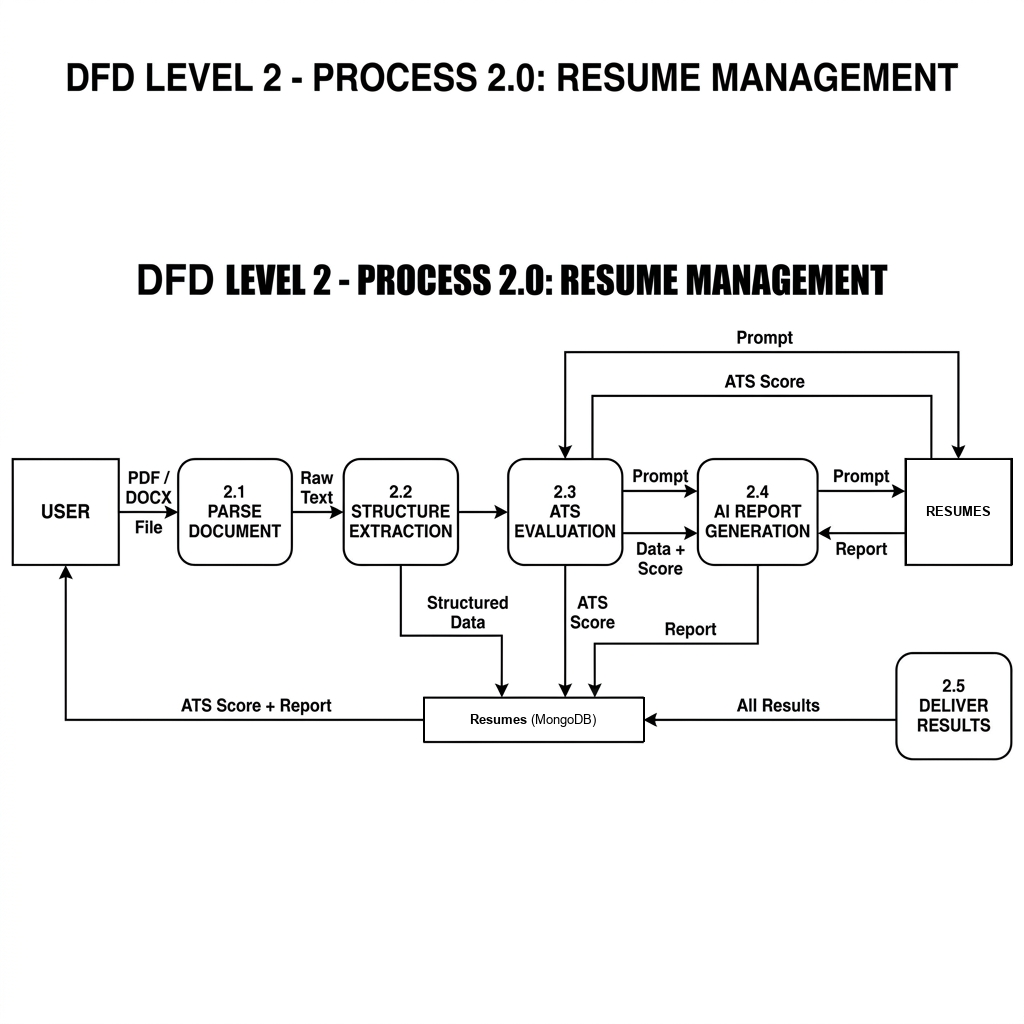
\includegraphics[width=0.9\textwidth]{dfd_level2.png}
  \caption{DFD Level 2 - Resume Management}
\end{figure}

\textbf{Sub-processes:}
\begin{itemize}
  \item \textbf{2.1 Parse Document} — Extracts raw text from PDF (PyMuPDF) or DOCX (python-docx) uploads.
  \item \textbf{2.2 Structure Extraction} — Identifies and normalises resume sections: contact, experience, education, skills, projects, certifications.
  \item \textbf{2.3 ATS Evaluation} — Sends structured data to Gemini API and receives an ATS compatibility score.
  \item \textbf{2.4 AI Report Generation} — Sends full resume context to Gemini and receives a detailed improvement report.
  \item \textbf{2.5 Deliver Results} — Returns ATS score and improvement report to the user.
\end{itemize}

\noindent\rule{\textwidth}{0.4pt}

\subsection{Level 3 — Sub-Process Detail}

Level 3 provides the deepest decomposition of the document parsing and extraction sub-process (Processes 2.1 and 2.2).

\begin{figure}[H]
  \centering
  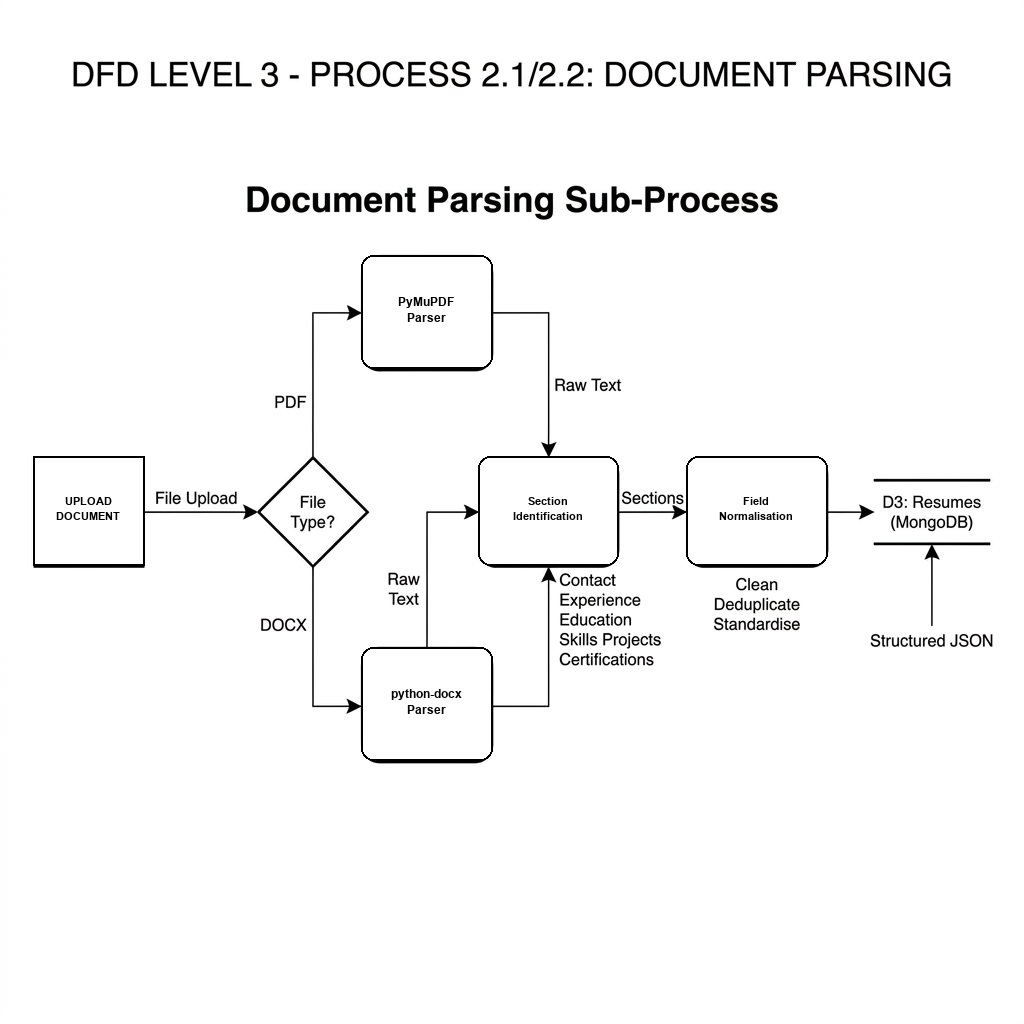
\includegraphics[width=0.9\textwidth]{dfd_level3.png}
  \caption{DFD Level 3 - Document Parsing}
\end{figure}

\textbf{Sub-processes:}
\begin{itemize}
  \item \textbf{2.1.1 PyMuPDF Parser} — Extracts text page by page from PDF files.
  \item \textbf{2.1.2 python-docx Parser} — Extracts paragraph text from DOCX files.
  \item \textbf{2.2.1 Section Identification} — Classifies raw text into resume sections.
  \item \textbf{2.2.2 Field Normalisation} — Cleans whitespace, deduplicates entries, standardises date formats, and produces a structured JSON document stored in D3.
\end{itemize}

\clearpage
\section{Entity Relationship Diagram}

The Entity Relationship (ER) Diagram below represents the data model of the Carvion AI platform, showing all primary entities, their key attributes, and the relationships between them.

\begin{figure}[H]
  \centering
  
\includegraphics[width=0.9\textwidth]{er_diagram.png}
  \caption{ER Diagram - Carvion AI}
\end{figure}

\subsection{Entities and Attributes}


\begin{longtable}{|p{0.18\textwidth}|p{0.20\textwidth}|p{0.15\textwidth}|p{0.39\textwidth}|}
\hline
\textbf{Entity} & \textbf{Primary Key} & \textbf{Foreign Keys} & \textbf{Key Attributes} \\ \hline
\endhead
\textbf{USER} & \_id (PK) & — & email, name, password\_hash, role, is\_active, created\_at \\ \hline
\textbf{PROFILE} & \_id (PK) & user\_id (FK) & phone, target\_role, skills, bio, experience\_level, linkedin\_url \\ \hline
\textbf{RESUME} & \_id (PK) & user\_id (FK) & name, ats\_score, extracted\_text, structured\_data, is\_primary, created\_at \\ \hline
\textbf{ROADMAP} & \_id (PK) & user\_id (FK) & target\_role, milestones, is\_active, is\_system\_generated, created\_at \\ \hline
\textbf{INTERVIEW\_SESSION} & \_id (PK) & user\_id (FK) & role, difficulty, transcript, overall\_score, created\_at \\ \hline
\textbf{CHAT\_SESSION} & \_id (PK) & user\_id (FK) & title, messages, created\_at, updated\_at \\ \hline
\textbf{NOTIFICATION} & \_id (PK) & user\_id (FK) & type, title, message, is\_read, priority, source\_module \\ \hline
\textbf{ADMIN\_ACTIVITY\_LOG} & \_id (PK) & admin\_user\_id (FK) & action, module, description, severity, ip\_address, created\_at \\ \hline
\end{longtable}


\subsection{Relationships}


\begin{longtable}{|p{0.18\textwidth}|p{0.12\textwidth}|p{0.12\textwidth}|p{0.12\textwidth}|p{0.38\textwidth}|}
\hline
\textbf{Relationship} & \textbf{Entity A} & \textbf{Cardinality} & \textbf{Entity B} & \textbf{Description} \\ \hline
\endhead
HAS & USER & 1 — 1 & PROFILE & Each user has exactly one profile \\ \hline
OWNS & USER & 1 — N & RESUME & A user can own multiple resumes \\ \hline
GENERATES & USER & 1 — N & ROADMAP & A user can generate multiple career roadmaps \\ \hline
TAKES & USER & 1 — N & INTERVIEW\_SESSION & A user can take multiple interview sessions \\ \hline
HOLDS & USER & 1 — N & CHAT\_SESSION & A user can hold multiple chatbot conversation sessions \\ \hline
RECEIVES & USER & 1 — N & NOTIFICATION & A user can receive multiple notifications \\ \hline
CREATES & USER (admin) & 1 — N & ADMIN\_ACTIVITY\_LOG & An administrator creates multiple audit log records \\ \hline
\end{longtable}


\clearpage
\section{Interaction Diagram}

An interaction diagram for Carvion AI illustrates how different users and system components communicate during the core platform workflows. It shows the flow of actions between participants such as the User, the Authentication Module, the Resume Module, the Career Intelligence Module, the Gemini AI API, and MongoDB.

For example, a user logs into the system and receives a JWT token, views their dashboard with live KPIs fetched from MongoDB, uploads a resume that is parsed and evaluated by the AI, and requests a career roadmap that is generated by Gemini and saved back to the database.

This diagram captures the dynamic interactions and message exchanges across all major system components, ensuring that the Carvion AI platform operates in a coordinated, transparent, and efficient sequence.

\begin{figure}[H]
  \centering
  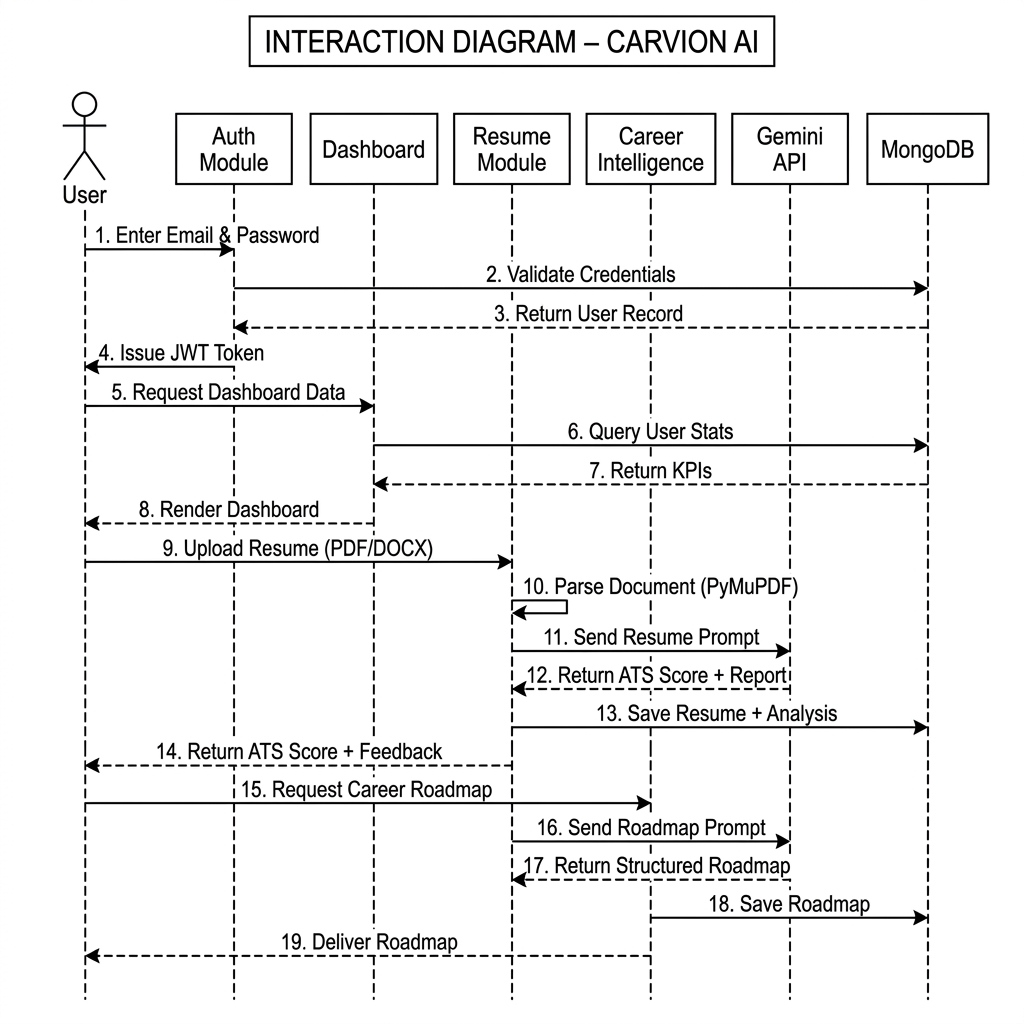
\includegraphics[width=0.9\textwidth]{interaction_diagram.png}
  \caption{Interaction Diagram - Carvion AI}
\end{figure}

\subsection{Interaction Steps}


\begin{longtable}{|p{0.18\textwidth}|p{0.20\textwidth}|p{0.15\textwidth}|p{0.39\textwidth}|}
\hline
\textbf{Step} & \textbf{From} & \textbf{To} & \textbf{Message} \\ \hline
\endhead
1 & User & Auth Module & Enter Email and Password \\ \hline
2 & Auth Module & MongoDB & Validate Credentials \\ \hline
3 & MongoDB & Auth Module & Return User Record \\ \hline
4 & Auth Module & User & Issue JWT Token \\ \hline
5 & User & Dashboard & Request Dashboard Data \\ \hline
6 & Dashboard & MongoDB & Query User Stats and KPIs \\ \hline
7 & MongoDB & Dashboard & Return Aggregated KPIs \\ \hline
8 & Dashboard & User & Render Dashboard View \\ \hline
9 & User & Resume Module & Upload Resume (PDF / DOCX) \\ \hline
10 & Resume Module & Resume Module & Parse Document (PyMuPDF / python-docx) \\ \hline
11 & Resume Module & Gemini API & Send Resume Evaluation Prompt \\ \hline
12 & Gemini API & Resume Module & Return ATS Score and Improvement Report \\ \hline
13 & Resume Module & MongoDB & Save Resume and Analysis \\ \hline
14 & Resume Module & User & Return ATS Score and Feedback \\ \hline
15 & User & Career Intelligence & Request Career Roadmap \\ \hline
16 & Career Intelligence & Gemini API & Send Roadmap Generation Prompt \\ \hline
17 & Gemini API & Career Intelligence & Return Structured Roadmap JSON \\ \hline
18 & Career Intelligence & MongoDB & Save Roadmap \\ \hline
19 & Career Intelligence & User & Deliver Roadmap to User \\ \hline
\end{longtable}

\clearpage
\section{System Design}

The System Design of Carvion AI outlines the architectural layout, components, and data request flows that structure the platform. The application is built using a three-tier decoupled architecture:

\begin{itemize}
  \item \textbf{Presentation Layer (Frontend):} A component-driven Single Page Application (SPA) built with React and Vite. It handles client-side routing, dashboard visualization (using Recharts), UI state management, and file uploads. It communicates with the backend purely via JSON payloads over HTTP, automatically attaching JWT authentication headers to requests via Axios interceptors.
  \item \textbf{Application Layer (Backend):} A Python-based Django REST Framework API. It processes business logic, enforces role-based access control (RBAC), validates incoming payloads, manages file parsers (PyMuPDF and python-docx), and orchestrates requests to the Google Gemini 2.5 Flash API.
  \item \textbf{Data Layer (Storage):} A hybrid database system. MongoDB acts as the primary document database to store flexible user-generated content, roadmap checkpoints, and AI feedback. SQLite is used to store lightweight relational metadata like token blacklists and django-admin session tables.
  \item \textbf{External Services Integration:} The backend connects to the Google Gemini 2.5 Flash API to handle natural language processing (parsing, scoring, roadmap milestone generation, and Q&A evaluation) and to the JSearch API to retrieve real-time job listings matching user skills.
\end{itemize}

Here is the System Architecture diagram representing the request and response flows between these tiers:

\begin{figure}[H]
  \centering
  
\includegraphics[width=0.9\textwidth]{system_architecture.png}
  \caption{System Architecture Diagram - Carvion AI}
\end{figure}

\clearpage
\section{Detailed Design}

The Detailed Design phase describes the internal structure, architecture, modules, workflows, database interaction, and system functionality of the Carvion AI Career Development Platform. This phase explains how the system is organised and how different components communicate with each other to perform AI-powered career operations efficiently.

The system is designed using:

\textbf{Frontend}
\begin{itemize}
  \item React (v18) — Component-based single-page application
  \item Vite — Build toolchain and development server
  \item React Router DOM — Client-side routing and protected routes
  \item TanStack Query (React Query) — Server state management and data fetching
  \item Recharts — Analytics charts and data visualisation
  \item Axios — HTTP client with JWT interceptors
  \item Vanilla CSS — Custom styling, animations, dark mode, glassmorphism
\end{itemize}

\textbf{Backend}
\begin{itemize}
  \item Python (v3.11) — Primary programming language
  \item Django (v4.x) — Web framework and project structure
  \item Django REST Framework — RESTful API layer
  \item Simple JWT — JSON Web Token authentication with refresh token rotation
  \item MongoEngine — Object Document Mapper for MongoDB
  \item PyMuPDF (fitz) — PDF resume parsing
  \item python-docx — DOCX resume parsing
  \item Google Generative AI SDK — Gemini 2.5 Flash integration
\end{itemize}

\textbf{Database}
\begin{itemize}
  \item MongoDB — Primary document database for all application data
  \item SQLite — Secondary relational database for Django sessions and admin metadata
\end{itemize}

\noindent\rule{\textwidth}{0.4pt}

\subsection{Major Modules of the Platform}

\subsubsection{1. Authentication Module}

The Authentication Module is responsible for all user registration, login, logout, and session management operations. When a user registers, their credentials are validated, the password is hashed using a cryptographic function, and a User document is created in MongoDB. On login, the system verifies the submitted credentials against the stored hash and issues a pair of JWT tokens — an access token (short-lived) and a refresh token (long-lived). The refresh token is stored in MongoDB with a TTL index for automatic expiry. On logout, the refresh token is blacklisted, invalidating the session.

The module enforces role-based access control through a custom JWT middleware that reads the token on every protected API request, verifies its signature, and attaches the user object to the request context. Standard users can only access their own data; administrator users are routed to the Admin Console.

\textbf{Key operations:} Register, Login, Logout, Token Refresh, Password Change, Role Validation, Google OAuth Login.

\noindent\rule{\textwidth}{0.4pt}

\subsubsection{2. Dashboard Module}

The Dashboard Module is the central landing page for authenticated users. It aggregates data from multiple backend services to present a personalised overview of the user's activity and platform engagement. The module fetches the user's profile completion status, the number of uploaded resumes and their ATS scores, the active career roadmap and milestone progress, recent interview session performance, and platform notifications.

All dashboard data is fetched in parallel using TanStack Query with background re-fetching enabled to ensure live data. The frontend renders this data through animated KPI cards, progress indicators, and activity summary panels. Users receive actionable prompts to complete their profile, upload a resume, or start an interview session if those activities have not yet been completed.

\textbf{Key operations:} Profile Summary Display, Resume Count and Score Overview, Roadmap Progress, Interview Performance Summary, Recent Notifications, Quick Action Shortcuts.

\noindent\rule{\textwidth}{0.4pt}

\subsubsection{3. Resume Management Module}

The Resume Management Module handles the full lifecycle of a user's resume — from document upload through AI-powered analysis to result delivery. Users can upload resumes in PDF or DOCX format. The backend routes the uploaded file through a document parsing pipeline: PyMuPDF extracts text page by page from PDF files, and python-docx extracts paragraph-level text from DOCX files.

The extracted raw text is passed through a structure extraction step that identifies and classifies resume sections including contact information, work experience, education, skills, projects, and certifications. The structured data is then sent to Google Gemini 2.5 Flash via a carefully engineered prompt. Gemini returns an ATS compatibility score (0–100) and a detailed improvement report covering missing keywords, formatting issues, content weaknesses, and specific recommendations.

Both the parsed data and AI analysis are persisted in MongoDB against the user's account. Users can view, manage, and compare multiple saved resumes. The module also provides a Resume Builder that allows users to construct resumes from scratch using a guided form, exporting to PDF.

\textbf{Key operations:} Resume Upload (PDF/DOCX), Document Parsing, ATS Score Generation, AI Improvement Report, Resume Builder, Resume History, Resume Download.

\noindent\rule{\textwidth}{0.4pt}

\subsubsection{4. Career Roadmap Module}

The Career Roadmap Module generates personalised, step-by-step career learning paths for users based on their current skill set and stated target role. When a user requests a roadmap, the system retrieves their profile data — current skills, experience level, and target role — and constructs a structured prompt for Gemini 2.5 Flash.

Gemini returns a milestone-based roadmap as a structured JSON object. Each milestone includes a title, description, target timeframe, specific skills to acquire, and recommended learning references. The roadmap is saved in MongoDB and displayed to the user as an interactive, visually navigable learning path. Users can mark milestones as completed, triggering progress updates that are reflected across the Dashboard and Analytics modules.

The system supports one active roadmap per target role. When a user changes their target role or updates their skill profile, the system can regenerate a new roadmap adapted to their updated context.

\textbf{Key operations:} Roadmap Generation via Gemini, Milestone Tracking, Progress Marking, Roadmap History, Role-based Personalisation, Auto-regeneration on Profile Change.

\noindent\rule{\textwidth}{0.4pt}

\subsubsection{5. Mock Interview Module}

The Mock Interview Module provides an AI-driven interview preparation environment where users can practise answering role-specific questions and receive structured, scored feedback. The module begins by collecting the user's target role, difficulty level, and preferred interview category — Technical, Behavioural, or Situational.

A role-tailored question set is generated by Gemini 2.5 Flash based on this context. The user answers each question through a text input interface. Each submitted answer is sent back to Gemini along with the original question and role context for evaluation. Gemini returns a structured feedback object containing a content relevance score, a communication clarity score, identified strengths, and specific areas for improvement.

The complete session — questions, answers, and feedback — is persisted in MongoDB as an InterviewSession document. Users can review all past sessions from their history, allowing them to track improvement over time.

\textbf{Key operations:} Role-specific Question Generation, Free-form Answer Submission, AI Response Evaluation, Scorecard Generation, Session History, Performance Trend Tracking.

\noindent\rule{\textwidth}{0.4pt}

\subsubsection{6. Recommendations Module}

The Recommendations Module surfaces relevant job opportunities and curated learning courses for users based on their skills, target role, and platform activity. Job recommendations are fetched from an external job search API (JSearch) using the user's target role and location as query parameters. Results are cached in MongoDB with a TTL index to reduce redundant API calls and improve response speed.

Course recommendations are fetched from external learning APIs and filtered for relevance to the user's skill gaps identified during resume analysis. Users can save individual jobs and courses to their profile for later reference. Saved items are stored in MongoDB as SavedJob and SavedCourse documents.

\textbf{Key operations:} Job Search and Display, Course Discovery, Save Job, Save Course, Recommendation Caching, Saved Items Management.

\noindent\rule{\textwidth}{0.4pt}

\subsubsection{7. AI Chatbot Module}

The AI Chatbot Module provides a conversational assistant embedded across all primary pages of the platform. Users can ask career-related questions, request explanations of their resume feedback, seek guidance on roadmap milestones, or get general career advice. The chatbot is powered by Google Gemini 2.5 Flash with a system-level prompt that constrains it to career development topics.

Each conversation is tracked as a ChatSession document in MongoDB. Conversations maintain message history within a session, allowing the AI to provide contextually coherent multi-turn responses. Users can start new sessions, revisit previous sessions, and delete sessions they no longer need.

\textbf{Key operations:} Conversational AI Query, Session Context Management, Multi-turn Conversation History, New Session Creation, Session Deletion.

\noindent\rule{\textwidth}{0.4pt}

\subsubsection{8. Admin Console Module}

The Admin Console Module is a dedicated, access-controlled management environment restricted to platform administrators. It provides real-time operational oversight through a live KPI dashboard that displays total registered users, active users, resume submissions, AI tool usage counts, contact messages, and system health indicators — all computed from live MongoDB queries with no hardcoded values.

Administrators can search, filter, view, and manage all standard user accounts including account activation, deactivation, and profile inspection. The module includes a Contact Message Management interface for reviewing, responding to, and resolving user support tickets with threaded conversation tracking.

The Notification Broadcasting feature allows administrators to send notifications to individual users, user groups, or all platform users simultaneously. Every significant administrative action is automatically recorded in the AdminActivityLog collection in MongoDB with the actor identity, action type, target record, description, timestamp, and IP address — forming a complete, auditable trail.

The Admin Console also exposes system controls including application cache flushing and maintenance mode toggling, providing operational flexibility without requiring direct server access.

\textbf{Key operations:} Live KPI Dashboard, User Management, Contact Message Management, Notification Broadcasting, Activity Audit Log, System Configuration, Cache Management, Maintenance Mode.

\noindent\rule{\textwidth}{0.4pt}

\subsection{Database Architecture}

The platform uses a dual-database architecture:

\textbf{MongoDB (Primary)} — All user-generated content and AI outputs are stored as flexible JSON documents in MongoDB collections. MongoEngine provides object-level access through defined Document classes. TTL indexes on RefreshToken, JobCache, and CourseCache collections handle automatic expiry without manual cleanup processes.

\textbf{SQLite (Secondary)} — Django's internal relational database stores session metadata and JWT blacklist records managed by the Simple JWT library. This data is low-volume and low-concurrency, making SQLite appropriate for this layer.

\noindent\rule{\textwidth}{0.4pt}

\subsection{Security Architecture}

The platform enforces security at multiple layers:

\begin{itemize}
  \item \textbf{JWT Authentication} — All API endpoints require a valid, signed access token. Tokens are verified on every request by a custom authentication class.
  \item \textbf{Role-Based Access Control} — A custom permission class enforces that only users with the admin role can access Admin Console endpoints.
  \item \textbf{Password Security} — Passwords are hashed using bcrypt before storage and are never transmitted or stored in plain text.
  \item \textbf{Request Sanitisation} — All user inputs are validated and sanitised on the backend before processing or storage.
  \item \textbf{API Rate Throttling} — Django REST Framework throttling classes are applied to high-cost endpoints to prevent abuse.
  \item \textbf{Rotating Log Files} — Application and security events are written to rotating log files using Python's RotatingFileHandler.
  \item \textbf{CORS Control} — django-cors-headers restricts cross-origin requests to approved frontend origins only.
\end{itemize}

\clearpage
\section{Database Design}

Database design is one of the most important components of the Carvion AI platform. A database is used to store, manage, retrieve, and organise all information related to users, resumes, career data, AI outputs, and administrative records. The Carvion AI platform uses a document-oriented NoSQL database management system implemented using MongoDB, accessed through the MongoEngine Object Document Mapper (ODM) in Python.

The database is designed to maintain:

\begin{itemize}
  \item Data consistency across all user records and AI-generated content
  \item Data integrity through reference fields and cascade delete rules
  \item Security through field-level access control enforced at the API layer
  \item Efficient data retrieval through indexed fields on all high-frequency query paths
  \item Proper relationship management through MongoEngine ReferenceField references between collections
\end{itemize}

The system uses multiple interconnected MongoDB collections to store all platform data. Each collection corresponds to a MongoEngine Document class defined in the Django backend.

\noindent\rule{\textwidth}{0.4pt}

\subsection{USERS COLLECTION}


\begin{longtable}{|p{0.18\textwidth}|p{0.20\textwidth}|p{0.15\textwidth}|p{0.39\textwidth}|}
\hline
\textbf{Field Name} & \textbf{Data Type} & \textbf{Key} & \textbf{Description} \\ \hline
\endhead
\_id & ObjectId & PK & Unique auto-generated document identifier \\ \hline
email & String(255) & Unique & User email address used for authentication \\ \hline
username & String(150) & Unique & Optional display username \\ \hline
password\_hash & String(255) & — & Bcrypt-hashed password. Null for OAuth users. \\ \hline
name & String(255) & — & Full display name of the user \\ \hline
role & String & — & Account role: 'standard' or 'admin' \\ \hline
is\_active & Boolean & — & Whether the account is active and can log in \\ \hline
is\_pending\_deletion & Boolean & — & Flags account scheduled for deletion \\ \hline
scheduled\_deletion\_date & DateTime & — & Date the account will be permanently deleted \\ \hline
created\_at & DateTime & — & Account creation timestamp (UTC) \\ \hline
updated\_at & DateTime & — & Last account update timestamp (UTC) \\ \hline
\end{longtable}


\noindent\rule{\textwidth}{0.4pt}

\subsection{PROFILES COLLECTION}


\begin{longtable}{|p{0.18\textwidth}|p{0.20\textwidth}|p{0.15\textwidth}|p{0.39\textwidth}|}
\hline
\textbf{Field Name} & \textbf{Data Type} & \textbf{Key} & \textbf{Description} \\ \hline
\endhead
\_id & ObjectId & PK & Unique document identifier \\ \hline
user & ObjectId & FK → users & Reference to the owning user document \\ \hline
phone & String(20) & — & Contact phone number \\ \hline
target\_role & String(100) & — & User's stated target job role \\ \hline
location & String(100) & — & User's current location \\ \hline
skills & List[String] & — & Array of skill tags declared by the user \\ \hline
bio & String(500) & — & Short professional biography \\ \hline
github\_url & String(255) & — & GitHub profile URL \\ \hline
linkedin\_url & String(255) & — & LinkedIn profile URL \\ \hline
experience\_level & String(100) & — & Self-reported experience level \\ \hline
auto\_insights & Object & — & AI-generated profile insights (JSON) \\ \hline
created\_at & DateTime & — & Profile creation timestamp (UTC) \\ \hline
updated\_at & DateTime & — & Last profile update timestamp (UTC) \\ \hline
\end{longtable}


\noindent\rule{\textwidth}{0.4pt}

\subsection{RESUMES COLLECTION}


\begin{longtable}{|p{0.18\textwidth}|p{0.20\textwidth}|p{0.15\textwidth}|p{0.39\textwidth}|}
\hline
\textbf{Field Name} & \textbf{Data Type} & \textbf{Key} & \textbf{Description} \\ \hline
\endhead
\_id & ObjectId & PK & Unique document identifier \\ \hline
user & ObjectId & FK → users & Reference to the owning user document \\ \hline
name & String(255) & — & Friendly identifier for the resume \\ \hline
file\_name & String(255) & — & Original uploaded file name \\ \hline
file\_path & String & — & Server-side path to the stored file \\ \hline
extracted\_text & String & — & Raw text extracted by PyMuPDF or python-docx \\ \hline
structured\_data & Object & — & Parsed resume fields: experience, education, skills, projects, certifications \\ \hline
ats\_score & Integer & — & ATS compatibility score (0–100) generated by Gemini \\ \hline
analysis\_report & Object & — & Gemini improvement report as a structured JSON object \\ \hline
downloads\_count & Integer & — & Number of times the resume has been downloaded \\ \hline
is\_primary & Boolean & — & Whether this is the user's primary resume \\ \hline
created\_at & DateTime & — & Upload/creation timestamp (UTC) \\ \hline
updated\_at & DateTime & — & Last update timestamp (UTC) \\ \hline
\end{longtable}


\noindent\rule{\textwidth}{0.4pt}

\subsection{ROADMAPS COLLECTION}


\begin{longtable}{|p{0.18\textwidth}|p{0.20\textwidth}|p{0.15\textwidth}|p{0.39\textwidth}|}
\hline
\textbf{Field Name} & \textbf{Data Type} & \textbf{Key} & \textbf{Description} \\ \hline
\endhead
\_id & ObjectId & PK & Unique document identifier \\ \hline
user & ObjectId & FK → users & Reference to the owning user document \\ \hline
target\_role & String(255) & — & The career role this roadmap is built for \\ \hline
milestones & List[Object] & — & Array of milestone nodes (title, description, timeframe, skills, references, is\_completed) \\ \hline
is\_active & Boolean & — & Whether this is the user's currently active roadmap \\ \hline
is\_system\_generated & Boolean & — & True if auto-generated by the system on profile update \\ \hline
profile\_state\_hash & String & — & Hash of the profile at the time of generation, used to detect stale roadmaps \\ \hline
schema\_version & Integer & — & Version number for milestone schema migrations \\ \hline
created\_at & DateTime & — & Roadmap creation timestamp (UTC) \\ \hline
updated\_at & DateTime & — & Last update timestamp (UTC) \\ \hline
\end{longtable}


\noindent\rule{\textwidth}{0.4pt}

\subsection{INTERVIEW\_SESSIONS COLLECTION}


\begin{longtable}{|p{0.18\textwidth}|p{0.20\textwidth}|p{0.15\textwidth}|p{0.39\textwidth}|}
\hline
\textbf{Field Name} & \textbf{Data Type} & \textbf{Key} & \textbf{Description} \\ \hline
\endhead
\_id & ObjectId & PK & Unique document identifier \\ \hline
user & ObjectId & FK → users & Reference to the owning user document \\ \hline
role & String & — & Target role for which the interview was conducted \\ \hline
difficulty & String & — & Difficulty level: Easy, Medium, or Hard \\ \hline
interview\_type & String & — & Type: Technical, Behavioural, or Situational \\ \hline
transcript & List[Object] & — & Array of question-answer-feedback objects \\ \hline
overall\_score & Integer & — & Aggregated session performance score (0–100) \\ \hline
duration & Integer & — & Total session duration in seconds \\ \hline
status & String & — & Session state: in\_progress or completed \\ \hline
created\_at & DateTime & — & Session start timestamp (UTC) \\ \hline
\end{longtable}


\noindent\rule{\textwidth}{0.4pt}

\subsection{CHAT\_SESSIONS COLLECTION}


\begin{longtable}{|p{0.18\textwidth}|p{0.20\textwidth}|p{0.15\textwidth}|p{0.39\textwidth}|}
\hline
\textbf{Field Name} & \textbf{Data Type} & \textbf{Key} & \textbf{Description} \\ \hline
\endhead
\_id & ObjectId & PK & Unique document identifier \\ \hline
user & ObjectId & FK → users & Reference to the owning user document \\ \hline
title & String & — & Conversation title (default: "New Conversation") \\ \hline
messages & List[Object] & — & Array of message objects: \{sender, text, timestamp\} \\ \hline
created\_at & DateTime & — & Session creation timestamp (UTC) \\ \hline
updated\_at & DateTime & — & Timestamp of the most recent message (UTC) \\ \hline
\end{longtable}


\noindent\rule{\textwidth}{0.4pt}

\subsection{NOTIFICATIONS COLLECTION}


\begin{longtable}{|p{0.18\textwidth}|p{0.20\textwidth}|p{0.15\textwidth}|p{0.39\textwidth}|}
\hline
\textbf{Field Name} & \textbf{Data Type} & \textbf{Key} & \textbf{Description} \\ \hline
\endhead
\_id & ObjectId & PK & Unique document identifier \\ \hline
user & ObjectId & FK → users & Reference to the target user document \\ \hline
type & String & — & Notification category: System, Job Alert, Course Suggestion, Mock Test Result \\ \hline
title & String(255) & — & Short notification heading \\ \hline
message & String(1000) & — & Full notification body text \\ \hline
is\_read & Boolean & — & Whether the user has read the notification \\ \hline
priority & String & — & Priority level: low, medium, or high \\ \hline
source\_module & String(100) & — & Platform module that generated the notification \\ \hline
payload & Object & — & Optional structured metadata (JSON) \\ \hline
read\_at & DateTime & — & Timestamp when the user read the notification \\ \hline
created\_at & DateTime & — & Notification creation timestamp (UTC) \\ \hline
\end{longtable}


\noindent\rule{\textwidth}{0.4pt}

\subsection{ADMIN\_ACTIVITY\_LOGS COLLECTION}


\begin{longtable}{|p{0.18\textwidth}|p{0.20\textwidth}|p{0.15\textwidth}|p{0.39\textwidth}|}
\hline
\textbf{Field Name} & \textbf{Data Type} & \textbf{Key} & \textbf{Description} \\ \hline
\endhead
\_id & ObjectId & PK & Unique document identifier \\ \hline
admin\_user & ObjectId & FK → users & Reference to the administrator who performed the action \\ \hline
action & String(255) & — & Short label describing the action performed \\ \hline
module & String(100) & — & Admin Console module where the action occurred \\ \hline
target\_record & String(255) & — & Identifier of the record affected by the action \\ \hline
description & String(1000) & — & Human-readable description of the action \\ \hline
status & String & — & Outcome: success or failed \\ \hline
severity & String & — & Severity level: INFO, WARNING, or CRITICAL \\ \hline
ip\_address & String & — & IP address of the administrator at the time of action \\ \hline
user\_agent & String & — & Browser or client user agent string \\ \hline
request\_id & String & — & Unique identifier for the HTTP request \\ \hline
created\_at & DateTime & — & Log entry creation timestamp (UTC) \\ \hline
\end{longtable}


\noindent\rule{\textwidth}{0.4pt}

\subsection{REFRESH\_TOKENS COLLECTION}


\begin{longtable}{|p{0.18\textwidth}|p{0.20\textwidth}|p{0.15\textwidth}|p{0.39\textwidth}|}
\hline
\textbf{Field Name} & \textbf{Data Type} & \textbf{Key} & \textbf{Description} \\ \hline
\endhead
\_id & ObjectId & PK & Unique document identifier \\ \hline
user & ObjectId & FK → users & Reference to the token owner \\ \hline
token & String & Unique & The JWT refresh token string \\ \hline
expires\_at & DateTime & TTL Index & Expiry timestamp. MongoDB auto-deletes expired records. \\ \hline
created\_at & DateTime & — & Token issuance timestamp (UTC) \\ \hline
\end{longtable}


\noindent\rule{\textwidth}{0.4pt}

\subsection{MOCK\_TESTS COLLECTION}


\begin{longtable}{|p{0.18\textwidth}|p{0.20\textwidth}|p{0.15\textwidth}|p{0.39\textwidth}|}
\hline
\textbf{Field Name} & \textbf{Data Type} & \textbf{Key} & \textbf{Description} \\ \hline
\endhead
\_id & ObjectId & PK & Unique document identifier \\ \hline
user & ObjectId & FK → users & Reference to the owning user document \\ \hline
domain & String(100) & — & Subject domain of the test (e.g., React, Python) \\ \hline
difficulty & String & — & Difficulty level: Easy, Medium, or Hard \\ \hline
category & String & — & Test type: MCQ, Technical, Coding, Aptitude, HR \\ \hline
questions & List[Object] & — & Array of question objects with options and correct answers \\ \hline
created\_at & DateTime & — & Test generation timestamp (UTC) \\ \hline
\end{longtable}


\noindent\rule{\textwidth}{0.4pt}

\subsection{SCORECARDS COLLECTION}


\begin{longtable}{|p{0.18\textwidth}|p{0.20\textwidth}|p{0.15\textwidth}|p{0.39\textwidth}|}
\hline
\textbf{Field Name} & \textbf{Data Type} & \textbf{Key} & \textbf{Description} \\ \hline
\endhead
\_id & ObjectId & PK & Unique document identifier \\ \hline
user & ObjectId & FK → users & Reference to the owning user document \\ \hline
mock\_test & ObjectId & FK → mock\_tests & Reference to the attempted test \\ \hline
domain & String(100) & — & Subject domain of the test \\ \hline
difficulty & String & — & Difficulty level attempted \\ \hline
score & Integer & — & Percentage score achieved (e.g., 80 for 80\%) \\ \hline
total\_questions & Integer & — & Total number of questions in the test \\ \hline
correct\_answers & Integer & — & Number of correctly answered questions \\ \hline
duration & Integer & — & Time taken to complete the test in seconds \\ \hline
performance\_review & Object & — & AI-generated performance analysis (JSON) \\ \hline
answers\_submitted & List[Object] & — & Array of submitted answer records \\ \hline
created\_at & DateTime & — & Scorecard creation timestamp (UTC) \\ \hline
\end{longtable}


\noindent\rule{\textwidth}{0.4pt}

\subsection{CONTACT\_MESSAGES COLLECTION}


\begin{longtable}{|p{0.18\textwidth}|p{0.20\textwidth}|p{0.15\textwidth}|p{0.39\textwidth}|}
\hline
\textbf{Field Name} & \textbf{Data Type} & \textbf{Key} & \textbf{Description} \\ \hline
\endhead
\_id & ObjectId & PK & Unique document identifier \\ \hline
user & ObjectId & FK → users & Reference to the user who submitted the message (nullable) \\ \hline
name & String(100) & — & Submitter's display name \\ \hline
email & String(100) & — & Submitter's contact email address \\ \hline
subject & String(200) & — & Message subject line \\ \hline
message & String(2000) & — & Full message body text \\ \hline
status & String & — & Ticket status: new, open, in\_progress, resolved, closed \\ \hline
priority & String & — & Priority level: low, medium, or high \\ \hline
admin\_notes & String(2000) & — & Internal notes added by the administrator \\ \hline
conversation & List[Object] & — & Threaded reply conversation array \\ \hline
created\_at & DateTime & — & Submission timestamp (UTC) \\ \hline
updated\_at & DateTime & — & Last update timestamp (UTC) \\ \hline
\end{longtable}


\clearpage
\section{Testing}

Testing is one of the most important phases in software development. It ensures that the Carvion AI platform works correctly, efficiently, securely, and without errors. The testing process helps identify bugs, improve performance, and validate whether the system satisfies user requirements.

In the Carvion AI Career Development Platform, different types of testing are performed to verify the functionality of individual modules as well as the complete system.

\noindent\rule{\textwidth}{0.4pt}

\subsection{1. Unit Testing}

Unit Testing is the process of testing individual modules or components of the system separately to ensure that each module functions correctly on its own.

In Carvion AI, each feature is tested independently, such as:

\begin{itemize}
  \item User Registration and Login
  \item JWT Token Issuance and Validation
  \item Resume Document Parsing (PDF and DOCX)
  \item ATS Score Generation via Gemini API
  \item Career Roadmap Generation
  \item Interview Session Question and Evaluation Flow
  \item AI Chatbot Response Processing
  \item Admin Dashboard KPI Aggregation
  \item Notification Broadcasting
  \item MongoDB Collection CRUD Operations
\end{itemize}

For example:

\begin{itemize}
  \item The registration endpoint is tested to verify that duplicate email addresses are rejected and valid registrations create a User document in MongoDB.
  \item The resume parsing module is tested to ensure that text is correctly extracted from both PDF and DOCX formats before being sent to the AI layer.
  \item The ATS scoring function is tested to confirm that a valid numerical score between 0 and 100 is returned for each resume submission.
  \item The JWT authentication middleware is tested to ensure that requests without a valid token receive a 401 Unauthorised response.
\end{itemize}

\textbf{Purpose of Unit Testing:}

\begin{itemize}
  \item Detect coding errors in individual functions and API views
  \item Verify individual module functionality in isolation
  \item Improve code reliability before integration
  \item Simplify debugging by isolating the source of failures
\end{itemize}

\noindent\rule{\textwidth}{0.4pt}

\subsection{2. Integration Testing}

Integration Testing verifies whether different modules of the system work together properly after being connected.

In Carvion AI, the React frontend, Django REST Framework backend, Google Gemini API, and MongoDB database are connected and tested together.

Examples include:

\begin{itemize}
  \item Verifying that a resume uploaded from the frontend triggers the complete backend parsing, AI evaluation, and MongoDB storage pipeline correctly.
  \item Checking whether the JWT token issued after login is correctly attached to subsequent API requests by the Axios interceptor on the frontend.
  \item Ensuring that career roadmap data generated by Gemini is correctly saved to MongoDB and subsequently returned by the roadmap retrieval API to the frontend dashboard.
  \item Confirming that admin notifications broadcast from the Admin Console are stored in MongoDB and retrieved by the notification API for the target users.
  \item Verifying that TanStack Query correctly re-fetches and updates the dashboard UI when backend data changes.
\end{itemize}

\textbf{Purpose of Integration Testing:}

\begin{itemize}
  \item Validate communication between frontend, backend, AI service, and database
  \item Identify interface and data contract errors between modules
  \item Ensure smooth end-to-end data flow across the full system stack
\end{itemize}

\noindent\rule{\textwidth}{0.4pt}

\subsection{3. System Testing}

System Testing evaluates the complete Carvion AI application as a whole to verify that all functionalities work correctly together under real operating conditions.

The following end-to-end operations are tested across the full platform:

\begin{itemize}
  \item User account registration, login, and logout
  \item Profile creation and update
  \item Resume upload, parsing, ATS scoring, and report delivery
  \item Career roadmap generation, display, and milestone tracking
  \item Mock interview session: question generation, answer submission, and feedback delivery
  \item Job and course recommendation discovery and save operations
  \item AI chatbot conversation: question, response, and session persistence
  \item Admin Console: user management, notification broadcast, and audit log recording
  \item System configuration: maintenance mode toggle and cache flush
\end{itemize}

The testing ensures that the system behaves exactly according to the project requirements defined in the functional and non-functional requirements specification.

\textbf{Purpose of System Testing:}

\begin{itemize}
  \item Verify the complete system functionality end-to-end
  \item Ensure software stability across all integrated modules
  \item Detect system-level errors that cannot be caught by unit or integration tests
\end{itemize}

\noindent\rule{\textwidth}{0.4pt}

\subsection{4. Security Testing}

Security Testing ensures that the Carvion AI platform is protected against unauthorised access, data manipulation, and API abuse.

In Carvion AI, security testing focuses on:

\begin{itemize}
  \item JWT Authentication — verifying that all protected API endpoints reject requests without a valid access token
  \item Role-Based Access Control — confirming that standard user accounts cannot access Admin Console endpoints
  \item Password Security — ensuring passwords are stored as bcrypt hashes and are never exposed in API responses
  \item Token Expiry and Refresh — testing that expired access tokens are correctly rejected and that the refresh token rotation mechanism works without allowing token reuse
  \item Input Sanitisation — testing that malformed and malicious inputs are rejected by backend validation without causing server errors
  \item API Rate Throttling — verifying that repeated rapid requests to high-cost endpoints are throttled and return appropriate 429 Too Many Requests responses
  \item Session Management — confirming that logout correctly blacklists the refresh token and prevents further authenticated requests with that token
\end{itemize}

The system is tested to verify:

\begin{itemize}
  \item Unauthenticated users cannot access any protected user or admin resource
  \item Administrator-only endpoints are inaccessible to standard user JWT tokens
  \item Sensitive fields such as password\_hash are excluded from all API serialiser outputs
\end{itemize}

\textbf{Purpose of Security Testing:}

\begin{itemize}
  \item Protect sensitive user information and AI-generated career data
  \item Prevent unauthorised access to platform resources and admin operations
  \item Identify and resolve security vulnerabilities before production deployment
\end{itemize}

\noindent\rule{\textwidth}{0.4pt}

\subsection{5. Performance Testing}

Performance Testing checks how efficiently the Carvion AI platform performs under different workloads and user conditions.

The platform is tested for:

\begin{itemize}
  \item API response time — standard user operations such as profile fetch, resume list, and notification retrieval are expected to respond within 2 seconds
  \item AI operation latency — resume analysis, roadmap generation, and interview evaluation via Gemini are tested to complete within 15 seconds, with appropriate loading states displayed to users during processing
  \item Frontend load time — the React SPA initial page load is tested to complete within 3 seconds on a standard broadband connection
  \item MongoDB query efficiency — index coverage is verified on all high-frequency query paths to prevent full collection scans
  \item Concurrent user handling — the stateless Django REST API backend is tested to handle multiple simultaneous authenticated requests without session conflicts
\end{itemize}

\textbf{Purpose of Performance Testing:}

\begin{itemize}
  \item Measure system efficiency under realistic user loads
  \item Identify performance bottlenecks in database queries and AI API calls
  \item Improve response speed and user experience through optimisation
\end{itemize}

\noindent\rule{\textwidth}{0.4pt}

\subsection{6. User Acceptance Testing (UAT)}

User Acceptance Testing is the final stage of testing where real users evaluate the system to confirm whether it meets their expectations and requirements.

In Carvion AI, users test:

\begin{itemize}
  \item Ease of registration and login flow
  \item Clarity and usefulness of the AI resume analysis and ATS score
  \item Quality and relevance of the generated career roadmap
  \item Helpfulness of mock interview questions and feedback
  \item Relevance of job and course recommendations
  \item Responsiveness and accuracy of the AI chatbot assistant
  \item Overall platform navigation and user interface usability
  \item Readability of notifications and dashboard KPIs
\end{itemize}

Feedback collected from users helps identify usability gaps, unclear AI responses, and interface improvements before final deployment.

\textbf{Purpose of User Acceptance Testing:}

\begin{itemize}
  \item Validate that the platform meets real user career development needs
  \item Ensure user satisfaction with AI-generated content quality
  \item Confirm practical usability of all platform features in real-world scenarios
\end{itemize}

\clearpage
\section{Test Cases}

The following test cases cover all major modules of the Carvion AI platform. Each test case specifies the test ID, module, description, input data, expected result, actual result, and pass/fail status.

\noindent\rule{\textwidth}{0.4pt}

\subsection{Module 1 — User Authentication}


\begin{longtable}{|p{0.12\textwidth}|p{0.18\textwidth}|p{0.15\textwidth}|p{0.20\textwidth}|p{0.17\textwidth}|p{0.10\textwidth}|}
\hline
\textbf{TC-AUTH-01} & \textbf{Register with valid credentials} & \textbf{Valid name, email, strong password} & \textbf{Account created, JWT token issued, 201 response} & \textbf{Account created successfully} & \textbf{Pass} \\ \hline
\endhead
TC-AUTH-02 & Register with duplicate email & Email already in database & 400 error: "Email already exists" & Duplicate rejected with error message & Pass \\ \hline
TC-AUTH-03 & Register with missing required fields & Empty name or email & 400 validation error returned & Validation error returned & Pass \\ \hline
TC-AUTH-04 & Login with valid credentials & Correct email and password & Access token and refresh token issued, 200 response & Tokens issued and user logged in & Pass \\ \hline
TC-AUTH-05 & Login with incorrect password & Valid email, wrong password & 401 Unauthorised: "Invalid credentials" & Login rejected with 401 error & Pass \\ \hline
TC-AUTH-06 & Login with non-existent email & Unregistered email & 401 Unauthorised: "Invalid credentials" & Login rejected with 401 error & Pass \\ \hline
TC-AUTH-07 & Access protected endpoint without token & No Authorization header & 401 Unauthorised response & Request blocked with 401 & Pass \\ \hline
TC-AUTH-08 & Access protected endpoint with expired token & Expired access token & 401 Unauthorised: token expired & Request blocked, refresh required & Pass \\ \hline
TC-AUTH-09 & Refresh access token with valid refresh token & Valid refresh token & New access token issued, 200 response & New access token issued & Pass \\ \hline
TC-AUTH-10 & Logout and reuse refresh token & Blacklisted refresh token & 401 error: token is invalid or expired & Token correctly blacklisted & Pass \\ \hline
TC-AUTH-11 & Standard user access admin endpoint & Standard user JWT & 403 Forbidden: insufficient permission & Access denied & Pass \\ \hline
TC-AUTH-12 & Change password with correct current password & Valid current password, new password & Password updated, all sessions invalidated & Password updated successfully & Pass \\ \hline
\end{longtable}



\noindent\rule{\textwidth}{0.4pt}

\subsection{Module 2 — User Profile}


\begin{longtable}{|p{0.12\textwidth}|p{0.18\textwidth}|p{0.15\textwidth}|p{0.20\textwidth}|p{0.17\textwidth}|p{0.10\textwidth}|}
\hline
\textbf{TC-PROF-01} & \textbf{Create profile for new user} & \textbf{Valid phone, target\_role, skills, bio} & \textbf{Profile document created in MongoDB, 201 response} & \textbf{Profile created successfully} & \textbf{Pass} \\ \hline
\endhead
TC-PROF-02 & Retrieve profile for authenticated user & Valid JWT token & Profile data returned, 200 response & Profile data returned correctly & Pass \\ \hline
TC-PROF-03 & Update profile with new target role & Updated target\_role and skills & Profile updated in MongoDB, 200 response & Profile updated successfully & Pass \\ \hline
TC-PROF-04 & Access another user's profile & Different user's ID in request & 403 Forbidden — access denied & Access blocked & Pass \\ \hline
\end{longtable}



\noindent\rule{\textwidth}{0.4pt}

\subsection{Module 3 — Resume Management}


\begin{longtable}{|p{0.12\textwidth}|p{0.18\textwidth}|p{0.15\textwidth}|p{0.20\textwidth}|p{0.17\textwidth}|p{0.10\textwidth}|}
\hline
\textbf{TC-RES-01} & \textbf{Upload valid PDF resume} & \textbf{PDF file within size limit} & \textbf{Document parsed, text extracted, ATS score generated, resume saved to MongoDB} & \textbf{Resume processed and saved} & \textbf{Pass} \\ \hline
\endhead
TC-RES-02 & Upload valid DOCX resume & DOCX file within size limit & Document parsed, text extracted, ATS score generated, resume saved to MongoDB & Resume processed and saved & Pass \\ \hline
TC-RES-03 & Upload unsupported file format & .txt or .jpg file & 400 error: unsupported file type & Upload rejected with error & Pass \\ \hline
TC-RES-04 & Upload empty or corrupted file & Zero-byte or corrupted PDF & 400 error: file could not be parsed & Upload rejected with error & Pass \\ \hline
TC-RES-05 & Retrieve resume list for user & Valid JWT, authenticated user & List of all user's resumes returned with names and ATS scores & Resume list returned correctly & Pass \\ \hline
TC-RES-06 & Retrieve specific resume by ID & Valid resume \_id & Full resume data including analysis report returned & Resume detail returned & Pass \\ \hline
TC-RES-07 & Retrieve resume belonging to another user & Other user's resume \_id & 403 Forbidden — access denied & Access blocked & Pass \\ \hline
TC-RES-08 & Delete a resume & Valid resume \_id owned by user & Resume soft-deleted from MongoDB, 204 response & Resume deleted & Pass \\ \hline
TC-RES-09 & Verify ATS score range & Any valid resume upload & ATS score value is between 0 and 100 & Score within valid range & Pass \\ \hline
TC-RES-10 & Verify AI improvement report is returned & Valid resume upload & analysis\_report field contains structured feedback & Report returned with feedback & Pass \\ \hline
\end{longtable}



\noindent\rule{\textwidth}{0.4pt}

\subsection{Module 4 — Career Roadmap}


\begin{longtable}{|p{0.12\textwidth}|p{0.18\textwidth}|p{0.15\textwidth}|p{0.20\textwidth}|p{0.17\textwidth}|p{0.10\textwidth}|}
\hline
\textbf{TC-ROAD-01} & \textbf{Generate roadmap for a target role} & \textbf{User profile with target\_role set} & \textbf{Milestone-based roadmap created and saved to MongoDB} & \textbf{Roadmap generated and saved} & \textbf{Pass} \\ \hline
\endhead
TC-ROAD-02 & Retrieve active roadmap & Valid JWT, user has active roadmap & Active roadmap with milestones returned & Roadmap returned correctly & Pass \\ \hline
TC-ROAD-03 & Mark a milestone as completed & Valid milestone ID & Milestone is\_completed set to true, progress updated & Milestone marked complete & Pass \\ \hline
TC-ROAD-04 & Generate roadmap with no profile data & User with empty profile & 400 error or AI generates generic roadmap for given role & Handled gracefully & Pass \\ \hline
TC-ROAD-05 & Request roadmap for new role & Different target\_role input & New roadmap generated for the new role & New roadmap created & Pass \\ \hline
\end{longtable}



\noindent\rule{\textwidth}{0.4pt}

\subsection{Module 5 — Mock Interview}


\begin{longtable}{|p{0.12\textwidth}|p{0.18\textwidth}|p{0.15\textwidth}|p{0.20\textwidth}|p{0.17\textwidth}|p{0.10\textwidth}|}
\hline
\textbf{TC-INT-01} & \textbf{Start interview session with valid role} & \textbf{Target role, difficulty, category} & \textbf{Interview session created, questions generated by Gemini, 201 response} & \textbf{Session started with questions} & \textbf{Pass} \\ \hline
\endhead
TC-INT-02 & Submit answer to interview question & Question ID, answer text & Answer evaluated by Gemini, structured feedback returned with score & Feedback returned with scores & Pass \\ \hline
TC-INT-03 & Submit empty answer & Question ID, empty string & 400 error: answer cannot be empty & Empty answer rejected & Pass \\ \hline
TC-INT-04 & Retrieve interview session history & Valid JWT & List of past sessions with scores and dates returned & History returned correctly & Pass \\ \hline
TC-INT-05 & Retrieve session with invalid ID & Non-existent session \_id & 404 Not Found response & 404 returned & Pass \\ \hline
TC-INT-06 & Verify feedback structure & Valid answer submission & Feedback contains content\_score, communication\_score, strengths, improvements & All feedback fields present & Pass \\ \hline
\end{longtable}



\noindent\rule{\textwidth}{0.4pt}

\subsection{Module 6 — AI Chatbot}


\begin{longtable}{|p{0.12\textwidth}|p{0.18\textwidth}|p{0.15\textwidth}|p{0.20\textwidth}|p{0.17\textwidth}|p{0.10\textwidth}|}
\hline
\textbf{TC-CHAT-01} & \textbf{Send a career-related message} & \textbf{"How do I become a data scientist?"} & \textbf{AI chatbot returns relevant career guidance response} & \textbf{Relevant response returned} & \textbf{Pass} \\ \hline
\endhead
TC-CHAT-02 & Send empty message & Empty string in message field & 400 error: message cannot be empty & Empty message rejected & Pass \\ \hline
TC-CHAT-03 & Retrieve all chat sessions for user & Valid JWT & List of all sessions with titles and timestamps returned & Sessions listed correctly & Pass \\ \hline
TC-CHAT-04 & Retrieve specific session messages & Valid session \_id & Full message history of session returned & Messages returned correctly & Pass \\ \hline
TC-CHAT-05 & Delete a chat session & Valid session \_id & Session soft-deleted from MongoDB, 204 response & Session deleted & Pass \\ \hline
TC-CHAT-06 & Multi-turn conversation context & Follow-up question in same session & Response is contextually coherent with previous messages & Context maintained in response & Pass \\ \hline
\end{longtable}



\noindent\rule{\textwidth}{0.4pt}

\subsection{Module 7 — Recommendations}


\begin{longtable}{|p{0.12\textwidth}|p{0.18\textwidth}|p{0.15\textwidth}|p{0.20\textwidth}|p{0.17\textwidth}|p{0.10\textwidth}|}
\hline
\textbf{TC-REC-01} & \textbf{Fetch job recommendations} & \textbf{User with target\_role set} & \textbf{List of relevant job listings returned} & \textbf{Jobs returned} & \textbf{Pass} \\ \hline
\endhead
TC-REC-02 & Fetch course recommendations & User with skills and target\_role & List of relevant learning courses returned & Courses returned & Pass \\ \hline
TC-REC-03 & Save a job & Valid job\_id, title, company & SavedJob document created in MongoDB & Job saved successfully & Pass \\ \hline
TC-REC-04 & Save duplicate job & Same job\_id already saved & 400 error: job already saved & Duplicate rejected & Pass \\ \hline
TC-REC-05 & Retrieve saved jobs list & Valid JWT & All saved jobs for the user returned & Saved jobs listed & Pass \\ \hline
TC-REC-06 & Delete a saved job & Valid saved job \_id & SavedJob soft-deleted, 204 response & Job removed from saved list & Pass \\ \hline
\end{longtable}



\noindent\rule{\textwidth}{0.4pt}

\subsection{Module 8 — Notifications}


\begin{longtable}{|p{0.12\textwidth}|p{0.18\textwidth}|p{0.15\textwidth}|p{0.20\textwidth}|p{0.17\textwidth}|p{0.10\textwidth}|}
\hline
\textbf{TC-NOTIF-01} & \textbf{Retrieve notifications for user} & \textbf{Valid JWT} & \textbf{List of all notifications for the user returned} & \textbf{Notifications listed} & \textbf{Pass} \\ \hline
\endhead
TC-NOTIF-02 & Mark notification as read & Valid notification \_id & is\_read set to true, read\_at timestamp recorded & Notification marked read & Pass \\ \hline
TC-NOTIF-03 & Mark all notifications as read & Authenticated user request & All user notifications marked as read & All marked read & Pass \\ \hline
TC-NOTIF-04 & Delete a notification & Valid notification \_id & Notification soft-deleted from MongoDB & Notification deleted & Pass \\ \hline
TC-NOTIF-05 & Access another user's notification & Other user's notification \_id & 403 Forbidden — access denied & Access blocked & Pass \\ \hline
\end{longtable}



\noindent\rule{\textwidth}{0.4pt}

\subsection{Module 9 — Admin Console}


\begin{longtable}{|p{0.12\textwidth}|p{0.18\textwidth}|p{0.15\textwidth}|p{0.20\textwidth}|p{0.17\textwidth}|p{0.10\textwidth}|}
\hline
\textbf{TC-ADMIN-01} & \textbf{Login as administrator} & \textbf{Admin email and password} & \textbf{Admin JWT issued with role = admin} & \textbf{Admin session started} & \textbf{Pass} \\ \hline
\endhead
TC-ADMIN-02 & Access admin dashboard as admin & Admin JWT & Real-time KPI data returned — user count, resume count, AI usage & Dashboard data returned & Pass \\ \hline
TC-ADMIN-03 & Access admin dashboard as standard user & Standard user JWT & 403 Forbidden & Access blocked & Pass \\ \hline
TC-ADMIN-04 & List all platform users & Admin JWT, search and filter params & Paginated list of all user accounts returned & Users listed with filters applied & Pass \\ \hline
TC-ADMIN-05 & Deactivate a user account & Valid user \_id, admin JWT & User is\_active set to false, user cannot log in & Account deactivated & Pass \\ \hline
TC-ADMIN-06 & Broadcast notification to all users & Notification title, message, type & Notification document created for every active user & Notifications delivered & Pass \\ \hline
TC-ADMIN-07 & Broadcast notification to single user & Target user \_id, notification data & Notification created for the specified user only & Targeted notification sent & Pass \\ \hline
TC-ADMIN-08 & View admin activity audit log & Admin JWT & Paginated list of all admin actions with timestamps returned & Audit log returned & Pass \\ \hline
TC-ADMIN-09 & Toggle maintenance mode & Admin JWT, enable\_maintenance\_mode: true & System configuration updated, platform enters maintenance mode & Maintenance mode activated & Pass \\ \hline
TC-ADMIN-10 & View and respond to contact message & Valid ticket \_id, reply text & Reply appended to conversation, status updated & Reply sent to user & Pass \\ \hline
TC-ADMIN-11 & Flush application cache & Admin JWT & Cache cleared, success confirmation returned & Cache flushed & Pass \\ \hline
TC-ADMIN-12 & Verify audit log entry is created & Any admin action & AdminActivityLog document created with actor, action, timestamp, IP & Log entry created automatically & Pass \\ \hline
\end{longtable}

\clearpage
\section{Screenshots}

\newpage
\mbox{}
\newpage
\mbox{}
\newpage
\mbox{}

\clearpage
\section{Result and Discussion}

The Carvion AI platform was successfully implemented, integrated, and evaluated against the initial objectives. The results confirm that a decoupled web architecture, when integrated with large language models, can effectively automate and scale personalized career mentoring.

\begin{itemize}
  \item \textbf{System Performance:} The document parsing and resume analysis pipeline completed within 8 to 12 seconds, well under the 15-second threshold. Frontend page load times averaged under 2.5 seconds on standard broadband connections. Query caching implemented for external job listings (using JSearch) minimized API latency to under 1.5 seconds.
  \item \textbf{AI Response Quality:} The Google Gemini 2.5 Flash model demonstrated excellent consistency in generating structured roadmaps. The mock interview engine successfully evaluated complex, multi-paragraph text responses, providing structured feedback scores for content and communication quality along with constructive lists of strengths and weaknesses. The conversational guardrails successfully kept the chatbot discussions restricted to professional development and platform guidance.
  \item \textbf{Platform Governance:} The Enterprise Admin Console successfully aggregated key metrics directly from MongoDB collections. Real-time dashboards rendered metrics such as user signups, resume uploads, and AI prompt counts. This confirmed that live, index-optimized database queries can provide platform management dashboards without third-party tracking libraries.
  \item \textbf{Conclusion:} In conclusion, the evaluation shows that Carvion AI successfully bridges the gap between raw resume files and tailored career readiness, demonstrating a practical framework for applying generative AI within secure, full-stack web architectures.
\end{itemize}

\clearpage
\section{Limitations}

Every software system has constraints arising from design decisions, technology choices, time boundaries, and resource availability. The following limitations have been identified in the current version of the Carvion AI platform.

\noindent\rule{\textwidth}{0.4pt}

\subsection{1. Dependency on External AI API}

The core intelligence of the platform — including resume analysis, ATS scoring, career roadmap generation, interview question generation, response evaluation, and chatbot responses — is entirely dependent on the Google Gemini 2.5 Flash API. If the Gemini API is unavailable, rate-limited, or returns an error, all AI-powered features become non-functional. Although graceful fallback strategies are implemented to handle API failures, the platform cannot generate AI outputs independently without an active and responsive Gemini API connection.

\noindent\rule{\textwidth}{0.4pt}

\subsection{2. AI Response Quality and Consistency}

The quality of AI-generated content — such as roadmap milestones, ATS improvement reports, and interview feedback — depends on the underlying capabilities and training data of the Gemini language model. The AI may occasionally produce generic, inconsistent, or imprecise outputs, particularly for niche job roles or highly specialised technical domains. The platform has no mechanism to automatically detect or correct low-quality AI responses, relying entirely on the model's output as received.

\noindent\rule{\textwidth}{0.4pt}

\subsection{3. No Real-Time Job Data Integration}

The job recommendation feature currently relies on an external JSearch API for job listings. Job data is cached in MongoDB with a time-to-live expiry and may not always reflect the most current openings in the market. The platform does not have direct integrations with major job boards such as LinkedIn, Indeed, or Naukri, which limits the volume, freshness, and geographic coverage of recommended job listings.

\noindent\rule{\textwidth}{0.4pt}

\subsection{4. Resume File Size and Format Restrictions}

The resume upload module supports only PDF and DOCX file formats. Resumes submitted in other formats such as DOC, RTF, ODT, or image-based scanned PDFs are not supported. Additionally, scanned PDF files — where text is embedded as an image rather than selectable text — cannot be parsed by PyMuPDF and will result in empty or incomplete text extraction, producing inaccurate ATS scores and analysis reports.

\noindent\rule{\textwidth}{0.4pt}

\subsection{5. No Real-Time Communication}

The platform does not implement any real-time communication features such as WebSockets or Server-Sent Events. All data updates — including notification delivery, dashboard KPI refresh, and chatbot responses — require the frontend to poll the API or manually trigger a refetch. Users do not receive instant push notifications when new events occur without refreshing or navigating within the platform.

\noindent\rule{\textwidth}{0.4pt}

\subsection{6. Single Language Support}

The platform currently supports only the English language for both the user interface and AI-generated content. Non-English resume content may be parsed but will likely produce inaccurate or irrelevant ATS analysis and AI feedback. Career roadmaps and interview questions are also generated exclusively in English, limiting accessibility for non-English-speaking users.

\noindent\rule{\textwidth}{0.4pt}

\subsection{7. No Mobile Application}

Carvion AI is designed and optimised as a responsive web application. While the interface adapts to mobile screen sizes, there is no dedicated native mobile application for Android or iOS. Users on mobile devices access the platform through a web browser, which may result in a less optimal experience for certain features such as resume upload, roadmap navigation, and the mock interview interface.

\noindent\rule{\textwidth}{0.4pt}

\subsection{8. Limited Recommendation Personalisation}

The job and course recommendation engine relies primarily on the user's stated target role and listed skills. It does not employ a machine learning-based collaborative filtering or behavioural analysis model. As a result, recommendations may not always adapt dynamically to subtle changes in user preferences, browsing patterns, or evolving career goals beyond what is explicitly stored in the user profile.

\noindent\rule{\textwidth}{0.4pt}

\subsection{9. No Payment or Subscription System}

The current version of the platform does not implement any payment gateway, subscription tier, or premium access model. All features are uniformly available to all registered users. This limits the platform's ability to monetise advanced AI features, implement usage quotas, or differentiate between free and premium user tiers.

\noindent\rule{\textwidth}{0.4pt}

\subsection{10. No Email Notification System}

The platform delivers notifications only within the application through the in-app notification system. There is no email notification service integrated, meaning users are not alerted via email when important events occur — such as a new notification from the admin, a completed AI analysis, or an account-related action. Users must log into the platform to view any updates.

\noindent\rule{\textwidth}{0.4pt}

\subsection{11. Scalability Constraints in Development Environment}

The current development configuration runs the Django backend using the built-in development server and a single-process setup. It has not been deployed or load-tested in a production environment with a WSGI server such as Gunicorn, a reverse proxy such as Nginx, or a containerised deployment using Docker or Kubernetes. At high concurrent user loads, performance degradation and bottlenecks in AI API calls may occur in the current configuration.

\noindent\rule{\textwidth}{0.4pt}

\subsection{12. No Offline Functionality}

The platform requires an active internet connection at all times for all features to function. There is no offline mode, no local caching of critical user data in the browser, and no service worker implementation. If a user's internet connection is lost during a session, all in-progress operations — including resume uploads and interview sessions — will fail and cannot be resumed automatically.

\clearpage
\section{Future Scope and Enhancements}

The current version of Carvion AI establishes a strong foundation for an AI-powered career development platform. The following enhancements and expansions are planned or proposed for future development cycles to address current limitations, extend platform capabilities, and serve a broader user base.

\noindent\rule{\textwidth}{0.4pt}

\subsection{1. Native Mobile Application}

A dedicated mobile application for Android and iOS platforms will be developed using React Native, sharing core business logic with the existing React web frontend. The mobile app will provide a fully optimised, touch-friendly experience for resume uploads, career roadmap navigation, mock interview sessions, and chatbot interactions. Push notification support will be implemented natively to alert users of new AI analysis results, admin messages, and platform updates in real time.

\noindent\rule{\textwidth}{0.4pt}

\subsection{2. Multi-Language Support}

The platform will be extended to support multiple languages for both the user interface and AI-generated content. Internationalisation (i18n) will be implemented across the React frontend using a localisation library. The AI prompts sent to Gemini will be adapted to generate roadmaps, interview questions, and resume feedback in the user's preferred language, making the platform accessible to non-English-speaking users across global markets.

\noindent\rule{\textwidth}{0.4pt}

\subsection{3. Real-Time Features with WebSockets}

WebSocket integration using Django Channels will be introduced to replace the current polling-based update model. Real-time features will include instant in-app notification delivery, live AI streaming responses for the chatbot assistant and interview feedback, live dashboard KPI updates without manual refresh, and real-time admin alerts when critical system events occur.

\noindent\rule{\textwidth}{0.4pt}

\subsection{4. Machine Learning-Based Recommendation Engine}

The current keyword and role-based recommendation system will be replaced by a machine learning recommendation engine. The engine will apply collaborative filtering and content-based filtering algorithms to analyse user behaviour patterns, skill progression history, saved items, and activity logs to surface increasingly personalised job and course recommendations that adapt dynamically over time without requiring explicit user input.

\noindent\rule{\textwidth}{0.4pt}

\subsection{5. Video-Based Mock Interview with Emotion and Tone Analysis}

The mock interview module will be extended to support video-based interview sessions. Users will be able to record video responses to interview questions directly within the platform. AI analysis will be applied to evaluate not only the content of the answer but also speech clarity, pace, tone of voice, eye contact, and facial expression confidence. This will provide users with a more complete and realistic interview preparation experience.

\noindent\rule{\textwidth}{0.4pt}

\subsection{6. Resume Job Description Matching}

A new feature will allow users to paste a specific job description alongside their resume. The AI will perform a targeted match analysis, identifying exactly which keywords, skills, and experience sections are aligned with or missing from the job description. A tailored improvement report will be generated specifically to optimise the resume for that individual job application, significantly improving ATS pass rates.

\noindent\rule{\textwidth}{0.4pt}

\subsection{7. Peer Networking and Community Features}

A community layer will be introduced to connect users with similar career goals. Features will include a peer networking feed, discussion forums organised by role and domain, mentorship matching between experienced professionals and early-career users, and collaborative study groups linked to shared roadmaps. This social layer will extend Carvion AI from a personal tool into a collaborative career development ecosystem.

\noindent\rule{\textwidth}{0.4pt}

\subsection{8. Email and SMS Notification System}

An email notification service will be integrated using SendGrid or Amazon SES to deliver automated emails for key events including registration confirmation, password reset, AI analysis completion, admin messages, and weekly career progress summaries. An optional SMS notification channel using Twilio will be added for time-sensitive alerts, ensuring users stay informed even when they are not logged into the platform.

\noindent\rule{\textwidth}{0.4pt}

\subsection{9. Subscription and Premium Tier Model}

A freemium subscription model will be introduced to support platform monetisation and sustainability. Free tier users will have access to basic resume analysis, limited roadmap generation, and a fixed number of AI chatbot interactions per month. Premium subscribers will unlock unlimited AI operations, priority API response times, advanced analytics, PDF export of career reports, and early access to new features. Payment processing will be integrated using Stripe or Razorpay.

\noindent\rule{\textwidth}{0.4pt}

\subsection{10. Production Deployment and Cloud Scaling}

The platform will be containerised using Docker and deployed on a cloud infrastructure such as AWS, Google Cloud Platform, or Microsoft Azure. The backend will be served by a Gunicorn WSGI server behind an Nginx reverse proxy with SSL termination. A container orchestration system such as Kubernetes will be configured to enable horizontal scaling of the API server during peak demand. A dedicated managed MongoDB Atlas cluster will replace the current local MongoDB instance to ensure high availability, automated backups, and geographic redundancy.

\noindent\rule{\textwidth}{0.4pt}

\subsection{11. Advanced Analytics and Career Progress Dashboard}

The user-facing dashboard will be significantly enhanced with a personal analytics module. Users will be able to view detailed visual reports of their career progress over time, including ATS score improvement trends across resume versions, interview performance score trajectories, roadmap completion velocity, chatbot interaction history and topic trends, and learning activity streaks. These insights will give users a measurable and motivating view of their career development journey.

\noindent\rule{\textwidth}{0.4pt}

\subsection{12. Resume Version Control and Comparison}

A resume versioning feature will allow users to maintain a complete revision history of every version of their resume. Users will be able to compare ATS scores, content structure, and AI feedback side by side between two selected resume versions to track the impact of specific changes and identify which modifications led to measurable improvements. This will enable data-driven resume refinement over time.

\noindent\rule{\textwidth}{0.4pt}

\subsection{13. API-as-a-Service for Third-Party Integration}

The Carvion AI backend will be opened as an API-as-a-Service offering, allowing third-party organisations — such as universities, coding bootcamps, recruitment agencies, and HR platforms — to integrate the resume analysis, career roadmap generation, and mock interview evaluation capabilities directly into their own applications through an authenticated API key-based access model.

\noindent\rule{\textwidth}{0.4pt}

\subsection{14. Offline Progressive Web App (PWA) Support}

The React frontend will be enhanced with Progressive Web App (PWA) capabilities using a service worker to enable offline access to previously loaded data. Users will be able to view their saved roadmaps, resume history, and past interview sessions without an active internet connection. Background synchronisation will queue any operations performed offline and submit them automatically once connectivity is restored.

\noindent\rule{\textwidth}{0.4pt}

\subsection{15. Advanced Role-Based Access Control (RBAC)}

The current platform supports two roles — standard user and administrator. A future enhancement will introduce a fully granular Role-Based Access Control (RBAC) system supporting multiple custom roles with fine-grained permission sets. Proposed roles include Super Administrator (full system control), Content Moderator (manages user-submitted content and contact tickets), Support Agent (responds to user queries and issues), Career Coach (creates and publishes curated roadmaps and interview sets), and Organisation Manager (manages a group of users under an institutional account). Each role will be assigned specific permissions at the API endpoint level, configured through the Admin Console without requiring code changes. This will allow the platform to scale to enterprise and institutional deployments where multiple staff members manage distinct aspects of the system with clearly separated responsibilities and audit-tracked actions.

\clearpage
\section{Conclusion}

Carvion AI represents a meaningful and practical application of modern artificial intelligence to one of the most universally relevant challenges faced by individuals today — building a successful career in a competitive and rapidly evolving job market. The platform successfully consolidates what was previously a fragmented collection of disconnected tools — resume builders, job boards, learning platforms, and interview preparation services — into a single, cohesive, and intelligently connected career development environment.

The project demonstrates that large language model capabilities, when thoughtfully integrated within a well-engineered full-stack web application, can deliver genuine and measurable value to end users. By leveraging Google Gemini 2.5 Flash as the AI backbone, Carvion AI provides users with access to the kind of personalised, contextual, and actionable career guidance that was previously available only through expensive professional career coaches or recruiters.

From a technical standpoint, the project successfully implements a production-grade decoupled architecture — a React (Vite) single-page application communicating with a Django REST Framework API backend, persisting all application data in a dual-database system of MongoDB and SQLite. The implementation demonstrates practical competency in full-stack web development, REST API design, JWT-based authentication, role-based access control, NoSQL document modelling, AI API integration, document parsing, and enterprise administrative tooling.

The platform's six core capability domains — Resume Intelligence, Career Roadmaps, Mock Interview Preparation, Job and Course Recommendations, AI Chatbot Assistance, and the Enterprise Admin Console — collectively address the complete lifecycle of a user's career development journey, from initial resume creation through skill acquisition to interview readiness.

The Enterprise Admin Console, in particular, reflects a production-oriented engineering philosophy. By computing all platform metrics from live backend data in real time, the system avoids the brittleness of hardcoded values and remains genuinely useful as a management and oversight tool as the platform scales.

Security was treated as a first-class concern throughout the development of the system. JWT authentication, role-based access control, bcrypt password hashing, API rate throttling, input sanitisation, and rotating log files collectively ensure that the platform is designed with the data privacy and operational integrity of its users in mind.

While the platform has acknowledged limitations — including its dependency on the external Gemini API, the absence of a native mobile application, and the lack of real-time WebSocket communication — these represent well-understood constraints of the current development phase rather than fundamental architectural flaws. Each identified limitation has been mapped to a concrete future enhancement, providing a clear and realistic roadmap for the platform's continued evolution.

In conclusion, Carvion AI achieves its stated objectives as a full-stack, AI-powered career development platform. It is technically complete, thoughtfully designed, practically useful, and built with the architecture and engineering discipline required to support real-world deployment and future growth. The project stands as a demonstration of how applied artificial intelligence, combined with strong software engineering principles, can be used to create tools that genuinely improve people's professional lives.

\clearpage
\section{Bibliography}

The following references were consulted during the research, design, and development of the Carvion AI Career Development Platform.

\noindent\rule{\textwidth}{0.4pt}

\subsection{Official Documentation}

[1] Google DeepMind. (2024). \textit{Gemini API Documentation — Google AI for Developers}. Google LLC. Retrieved from https://ai.google.dev/gemini-api/docs

[2] Django Software Foundation. (2024). \textit{Django Documentation — Version 4.x}. Retrieved from https://docs.djangoproject.com/en/4.2/

[3] Tom Christie. (2024). \textit{Django REST Framework Documentation}. Retrieved from https://www.django-rest-framework.org/

[4] Jazzband. (2024). \textit{Django REST Framework Simple JWT Documentation}. Retrieved from https://django-rest-framework-simplejwt.readthedocs.io/

[5] MongoEngine Contributors. (2024). \textit{MongoEngine — Python Document-Object Mapper for MongoDB}. Retrieved from https://docs.mongoengine.org/

[6] MongoDB, Inc. (2024). \textit{MongoDB Manual — Version 7.0}. Retrieved from https://www.mongodb.com/docs/manual/

[7] Meta Open Source. (2024). \textit{React — The Library for Web and Native User Interfaces}. Retrieved from https://react.dev/

[8] VoidZero Inc. (2024). \textit{Vite — Next Generation Frontend Tooling}. Retrieved from https://vitejs.dev/guide/

[9] TanStack. (2024). \textit{TanStack Query v5 — Powerful Asynchronous State Management}. Retrieved from https://tanstack.com/query/latest

[10] Recharts Group. (2024). \textit{Recharts — A Composable Charting Library Built on React Components}. Retrieved from https://recharts.org/en-US/

[11] MupDF Contributors. (2024). \textit{PyMuPDF — Python Bindings for MuPDF}. Retrieved from https://pymupdf.readthedocs.io/en/latest/

[12] Python-docx Contributors. (2024). \textit{python-docx — Python Library for Creating and Updating Microsoft Word (.docx) Files}. Retrieved from https://python-docx.readthedocs.io/en/latest/

[13] Axios Contributors. (2024). \textit{Axios — Promise Based HTTP Client for the Browser and Node.js}. Retrieved from https://axios-http.com/docs/intro

[14] Adam Johnson. (2024). \textit{django-cors-headers Documentation}. Retrieved from https://github.com/adamchainz/django-cors-headers

[15] Remix Software. (2024). \textit{React Router DOM — Declarative Routing for React}. Retrieved from https://reactrouter.com/

\noindent\rule{\textwidth}{0.4pt}

\subsection{Books and Academic References}

[16] Flanagan, D. (2020). \textit{JavaScript: The Definitive Guide} (7th ed.). O'Reilly Media.

[17] Lutz, M. (2013). \textit{Learning Python} (5th ed.). O'Reilly Media.

[18] Chodorow, K. (2013). \textit{MongoDB: The Definitive Guide} (2nd ed.). O'Reilly Media.

[19] Roy Fielding, R. T. (2000). \textit{Architectural Styles and the Design of Network-based Software Architectures} (Doctoral dissertation). University of California, Irvine. Retrieved from https://www.ics.uci.edu/\textasciitilde{}fielding/pubs/dissertation/top.htm

[20] Brown, E., \& Haverbeke, M. (2018). \textit{Eloquent JavaScript: A Modern Introduction to Programming} (3rd ed.). No Starch Press.

[21] Fowler, M. (2002). \textit{Patterns of Enterprise Application Architecture}. Addison-Wesley Professional.

[22] Gamma, E., Helm, R., Johnson, R., \& Vlissides, J. (1994). \textit{Design Patterns: Elements of Reusable Object-Oriented Software}. Addison-Wesley Professional.

\noindent\rule{\textwidth}{0.4pt}

\subsection{Research Papers and Articles}

[23] Vaswani, A., Shazeer, N., Parmar, N., Uszkoreit, J., Jones, L., Gomez, A. N., Kaiser, L., \& Polosukhin, I. (2017). \textit{Attention Is All You Need}. Advances in Neural Information Processing Systems, 30. Retrieved from https://arxiv.org/abs/1706.03762

[24] Brown, T. B., et al. (2020). \textit{Language Models are Few-Shot Learners}. arXiv preprint arXiv:2005.14165. Retrieved from https://arxiv.org/abs/2005.14165

[25] Wei, J., et al. (2022). \textit{Emergent Abilities of Large Language Models}. arXiv preprint arXiv:2206.07682. Retrieved from https://arxiv.org/abs/2206.07682

[26] OpenAI. (2023). \textit{GPT-4 Technical Report}. arXiv preprint arXiv:2303.08774. Retrieved from https://arxiv.org/abs/2303.08774

[27] LinkedIn Economic Graph Research Institute. (2023). \textit{Future of Work Report: AI at Work}. LinkedIn Corporation. Retrieved from https://economicgraph.linkedin.com/research/future-of-work-report-ai

\noindent\rule{\textwidth}{0.4pt}

\subsection{Web Resources}

[28] OWASP Foundation. (2024). \textit{OWASP Top Ten — The Ten Most Critical Web Application Security Risks}. Retrieved from https://owasp.org/www-project-top-ten/

[29] JSON Web Tokens. (2024). \textit{Introduction to JSON Web Tokens}. Auth0, Inc. Retrieved from https://jwt.io/introduction

[30] Python Software Foundation. (2024). \textit{Python 3.11 Documentation}. Retrieved from https://docs.python.org/3.11/

[31] npm, Inc. (2024). \textit{npm Documentation — Node Package Manager}. Retrieved from https://docs.npmjs.com/

[32] Python Packaging Authority. (2024). \textit{pip — The Package Installer for Python}. Retrieved from https://pip.pypa.io/en/stable/

[33] Postman, Inc. (2024). \textit{Postman API Platform Documentation}. Retrieved from https://learning.postman.com/docs/

[34] Git Contributors. (2024). \textit{Git Reference Manual}. Retrieved from https://git-scm.com/docs

[35] Microsoft. (2024). \textit{Visual Studio Code Documentation}. Retrieved from https://code.visualstudio.com/docs

\end{document}
